\documentclass[11pt]{article}
\usepackage[T1]{fontenc}
\usepackage[utf8]{inputenc}
\usepackage{lmodern}
\usepackage[margin=1in]{geometry}
\usepackage{amsmath,amssymb,graphicx,booktabs,longtable,tabularx,array}
\usepackage{microtype}
\usepackage[round,authoryear]{natbib}
\usepackage[font=small,labelfont=bf]{caption}
\usepackage[colorlinks=true,linkcolor=blue,citecolor=blue,urlcolor=blue]{hyperref}
\hypersetup{pdftitle={Recurring transit-like signals in six TESS fields},pdfauthor={Richard Higgins},pdfsubject={Exploratory candidate assessment; no validated planet}}
\graphicspath{{figures/}}
\setlength{\emergencystretch}{2em}
\setcounter{topnumber}{2}
\setcounter{bottomnumber}{2}
\setcounter{totalnumber}{4}
\renewcommand{\topfraction}{0.9}
\renewcommand{\bottomfraction}{0.8}
\renewcommand{\textfraction}{0.08}
\renewcommand{\floatpagefraction}{0.7}
\newcommand{\evidence}[2]{\href{https://github.com/relh/exoplanet/tree/0537d585d/#1}{#2}}
\title{Recurring transit-like signals in six TESS fields:\\evidence, source ambiguity, and limits of validation}
\author{Richard Higgins\\\small\href{mailto:richard@relh.net}{richard@relh.net}}
\date{20 October 2026\\\small Preprint draft; scientific evidence assessed through 13 October 2026}
\begin{document}
\maketitle
\begin{abstract}
We report an exploratory search and assessment of six transit-like signals in public TESS photometry. The strongest recurring signals are associated with the catalog fields of TIC~80387959 and TIC~402358350, at investigated periods of 4.19217 and 11.76954 days. A clock fixed before inspecting two later epochs of TIC~80387959 recovers dimming of $621\pm98$ and $651\pm114$ parts per million (ppm). Retrospective local-baseline fits retain positive depths in six sectors. For TIC~402358350, eight usable events remain positive under twelve local-baseline choices, with combined depths of 590--659 ppm. Its later-sector timing uncertainty fails the declared prediction gate. Neither signal has secure source attribution: neighboring stars can supply the missing flux, image models fail shallow known-host controls, and conditional astrophysical scenario calculations do not meet the joint validation thresholds. The other four signals retain single-epoch physical degeneracy, weak or timing-dependent recurrence, or evidence favoring contamination. We provide the adopted clocks, event and processing comparisons, control failures, alternative explanations, and a linked evidence inventory with file hashes. The overlapping searches and selected injections do not establish survey completeness or calibrated false-alarm rates. These results identify follow-up questions rather than validated planets, and catalog non-matches do not establish novelty.
\end{abstract}

\section{Introduction}
Public photometry from the Transiting Exoplanet Survey Satellite (TESS; \citealt{ricker2015}) allows searches for repeated dimming beyond the mission's original target lists. A recurring dip is an observable pattern; its astrophysical interpretation requires identifying the star that dims and distinguishing a planetary transit from stellar eclipses, blended variability, and instrumental effects. Repeating a measurement with another reduction of the same exposures tests processing sensitivity but does not supply independent observing evidence.

This paper documents six unresolved signals retained from several related searches. We prioritize TIC~80387959 and TIC~402358350 because their dimming persists across multiple epochs and analysis choices. We also retain the unfavorable evidence that prevents a planetary conclusion. The remaining fields---TIC~241928959, TIC~469309982, TIC~96166003, and TIC~5546257---illustrate distinct limitations rather than four additional validated discoveries. The designation ``ambiguous planetary candidate'' (APC), used in the accompanying research archive, is an internal working category. It is neither an official TESS Object of Interest designation nor a probability statement. TIC~5546257 is retained for its instructive contamination evidence, while its on-target planet interpretation is deprioritized.

Our contribution is an auditable record of the investigated signals and decision rules. It includes failed predictions, unusable observations, negative controls, and superseded interpretations. The six signals were not all selected from one homogeneous survey, so their number cannot be divided by a single target count to estimate occurrence. No signal is claimed as a newly validated or confirmed planet. Methods and control outcomes appear in Section~\ref{sec:methods}, the two priority fields in Section~\ref{sec:primary}, and the remaining fields in Section~\ref{sec:other}.

\section{Data and signal inventory}\label{sec:data}
We use public TESS-SPOC and Quick-Look Pipeline (QLP) products obtained through MAST \citep{caldwell2020,huang2020}. The saved run records identify the product, sector, flux column, quality selection, timestamp convention, retrieval location, and raw-content SHA-256. Simple-aperture photometry (SAP) and presearch-data-conditioning photometry (PDCSAP, abbreviated PDC below) are reductions of the same exposures. Likewise, QLP and SPOC products for an overlapping sector share observing photons. They are useful processing comparisons, not independent astronomical confirmations. QLP extraction changed from sector~94 \citep{petitpas2026}; an apparent inter-sector depth change cannot be assigned a physical origin without addressing extraction, sampling, and dilution.

Table~\ref{tab:inventory} summarizes the examined epochs and a representative later or local measurement. An ``opened'' sector has already been inspected in this investigation; the label does not establish adequate coverage, successful recovery, or an independent holdout. The sector~64 and~99 cutouts requested for TIC~80387959 contain collateral pixels at the target aperture. They are unusable target observations, not transit non-detections. Metadata-only footprints for TIC~96166003/71 and TIC~5546257/8/63 remain untested and are excluded from the evidence counts.

\begin{table}[htbp]
\centering\small
\caption{Retained signals and representative evidence. Errors are conditional on the stated photometric model. A positive fixed-clock depth alone does not satisfy timing or source-attribution requirements.}\label{tab:inventory}
\begin{tabularx}{\textwidth}{@{}l l X X@{}}
\toprule
TIC & Examined usable sectors & Representative evidence & Principal limitation\\
\midrule
80387959 & 10,36,37,63,90,100 & Frozen later-sector depths $621\pm98$, $651\pm114$ ppm & Host and depth differences unresolved\\
402358350 & 40,41,54,81 & Eight local-baseline events; 590--659 ppm combined & Later timing gate fails; host uncertain\\
241928959 & 92 & Five events; local depth $11992\pm786$ ppm & One epoch; grazing/companion degeneracy\\
469309982 & 9,10,36,37,63,64,90 & Frozen sector 64: $76\pm26$ ppm; sector 90 primary: $-54\pm32$ ppm & Mixed, clock-dependent recurrence\\
96166003 & 19,43,44,59,86 & Frozen sector 59 primary: $265\pm52$ ppm & Alternative clocks disagree; timing fails\\
5546257 & 9,35,36,62,89,99 & Frozen sector 62: $386\pm30$ ppm; neighbor Gaia dimming & Contamination favored; exact alias unresolved\\
\bottomrule
\end{tabularx}
\end{table}

Catalog identities and positions are given in Table~\ref{tab:stars}. Gaia DR3 coordinates are ICRS at J2016.0 \citep{gaia2023}; observations at other dates require propagation where appropriate. TIC stellar parameters \citep{tic2019} characterize the catalog stars, without establishing that those stars host the dips. We deliberately do not report adopted planet radii or masses. Normal Gaia renormalized unit weight error (RUWE) and absent non-single-star solutions do not exclude unresolved companions. The elevated RUWE of TIC~241928959 is a concern, not a companion detection.

\begin{table}[htbp]
\centering\scriptsize
\caption{Catalog context for the named target stars. Coordinates are Gaia DR3 at J2016.0; $T$ magnitudes, temperatures and radii are TIC values. Symmetric errors summarize the stored catalog fields and do not encompass all stellar-model systematics.}\label{tab:stars}
\begin{tabular}{@{}l r r r r r r r@{}}
\toprule
TIC & Gaia DR3 source ID & RA (deg) & Dec (deg) & $T$ & $T_{\rm eff}$ (K) & $R_\star/R_\odot$ & RUWE\\
\midrule
80387959 & 5362389543781401216 & 165.310575 & $-48.613881$ & 10.524 & $5220\pm125$ & $0.797\pm0.045$ & 0.828\\
402358350 & 4318715445843296256 & 295.150929 & $+15.640412$ & 9.432 & $6079\pm138$ & $0.995\pm0.046$ & 1.000\\
241928959 & 6865254022910168320 & 297.986934 & $-21.503148$ & 12.614 & $3396\pm157$ & $0.651\pm0.020$ & 3.356\\
469309982 & 5259582389096040960 & 148.847729 & $-56.685744$ & 9.215 & $5445\pm125$ & $0.879\pm0.047$ & 0.978\\
96166003 & 161856980718462208 & 72.588533 & $+33.707024$ & 10.423 & $5171\pm237$ & $0.825\pm0.049$ & 0.983\\
5546257 & 5426593115802740992 & 143.087875 & $-40.474512$ & 9.588 & $5826\pm131$ & $0.925\pm0.045$ & 0.913\\
\bottomrule
\end{tabular}
\end{table}

\begin{table}[htbp]
\centering\small
\caption{Adopted reference clocks, rounded for display. BTJD is ${\rm BJD}_{\rm TDB}-2457000$. Values identify historical predictions, not unique orbital solutions or parameter precision. Full stored values and alternative hypotheses remain in the linked evidence. Durations are fixed box widths, not physical transit-duration posteriors.}\label{tab:clocks}
\begin{tabular}{@{}l r r r l@{}}
\toprule
TIC & $P$ (days) & $t_0$ (BTJD) & $D$ (days) & Training sectors\\
\midrule
80387959 & 4.192168718 & 1575.375831 & 0.092736 & 10,36,37,63\\
402358350 & 11.769544332 & 2392.992869 & 0.144000 & 40,41,54\\
241928959 & 3.532592898 & 3805.411657 & 0.032000 & 92\\
469309982 & 2.890464274 & 1545.740130 & 0.144000 & 9,10,36,37\\
96166003 & 0.955530474 & 1816.967196 & 0.059520 & 19,43,44\\
5546257 & 1.767290230 & 1545.965336 & 0.133056 & 9,35,36\\
\bottomrule
\end{tabular}
\end{table}

\section{Search, evidence preservation, and controls}
\label{sec:methods}

\subsection{Observations and search populations}

We searched public TESS photometry for recurring transit-like dimming
\cite{ricker2015}, using TESS-SPOC and Quick-Look Pipeline (QLP) products
\cite{caldwell2020,huang2020}. Target properties and initial contamination
estimates came from the TESS Input Catalog (TIC; \cite{tic2019}). The six
retained signals emerged from several successive, overlapping campaigns.
They are not six discoveries from a single uniform survey, and the denominators
in Table~\ref{tab:campaigns} must not be added to obtain a unique-star count.
The investigation was adaptive: later experiments responded to earlier
controls and candidate assessments. We report the executed selection and
its limitations rather than interpreting the final shortlist as a statistical
planet yield.

\begin{table}[htbp]
\centering
\small
\caption{Completed search scopes. Counts describe processing outcomes,
not astrophysical classifications. The weak-seed stars were already counted
in earlier searches; other scopes also overlap.}
\label{tab:campaigns}
\begin{tabularx}{\linewidth}{@{}l r X@{}}
\toprule
Scope & Attempts & Reconciled outcome \\
\midrule
Solar-radius pool & 7,004 & 4,481 below threshold; 2,494 flagged;
28 screening passes, all reviewed; one original data error. \\
Weak-seed refinement & 689 & 688 measurements and one error;
23 local flags, all reviewed; 22 deprioritized. \\
Faint QLP pilot & 100 & 46 below threshold; 54 flagged; no errors
or full screening passes. \\
Faint QLP expansion & 1,845 & 950 below threshold; 888 flagged;
seven original data failures. Six recoveries gave 1,844 usable searches;
17 peak follow-ups on 16 stars. \\
\bottomrule
\end{tabularx}
\end{table}

The solar-radius inventory selected catalog radii of
$0.81$--$1.10\,R_\odot$, TESS magnitudes $6$--$12$, and distances
up to 120~pc. Of 16,581 opportunities with early and later TESS-SPOC coverage,
408 were excluded by exact identifiers in saved planet, candidate, and
eclipsing-binary catalogs, 1,635 failed the contamination-ratio requirement
of at most 0.2 or lacked its value, and 7,534 lacked an adjacent early-sector
pair. The remaining 7,004 were ranked by
$R_\star^2 10^{0.2(T-10)}/\sqrt{N_{\rm train}}$.
This is a metadata-based noise proxy, not measured quietness.
The earliest contiguous group of two or three sectors numbered at most 55
trained discovery, while the latest available ordinary sector numbered
56--107 was reserved. No temperature cut was applied to this pool.

The fainter QLP pool used $12<T\leq13.5$, catalog radii
$0.15$--$0.5\,R_\odot$, distances up to 120~pc,
$T_{\rm eff}\leq4000$~K, and the same contamination-ratio limit.
Dated catalog exclusions, TIC quality dispositions, and prior raw-data
access were checked before selection. From 38,822 eligible metadata targets,
1,945 had a suitable four-sector sequence and a separate reserved epoch.
Discovery used the latest four consecutive QLP sectors ending no later
than sector 96; reserved sectors were at least eight sector numbers from
every training sector. Their actual training baseline could not exceed
120~days. Sector-number separation alone does not establish independent
or usable observations. The four-sector design followed limited known-planet
controls and was therefore an informed design change, not a blind survey
choice. The first 100 targets formed the pilot and the remaining 1,845 the
expansion. Six expansion failures were recovered with three usable assigned
sectors; one target remained unsearchable with only two. Recoveries are
neither additional stars nor equivalent to four-sector coverage.

\subsection{Preprocessing and recurring-dip search}

For TESS-SPOC we used corrected PDCSAP flux and its supplied errors.
We retained quality-zero samples with finite times and positive, finite fluxes
and uncertainties, sorted timestamps, and removed duplicate timestamps.
FITS identities, integrity information, raw-product URLs, retrieval records,
and SHA-256 hashes were retained. Times are expressed as
${\rm BTJD}={\rm BJD}_{\rm TDB}-2457000$.
QLP flux and error columns were recorded per product. Where a target's
explicitly enabled fallback encountered no usable published errors, it
assigned equal errors from the robust adjacent-difference scale,
$1.4826\,\operatorname{MAD}(\Delta f)/\sqrt{2}$.
This estimates short-timescale scatter rather than a calibrated correlated-noise
uncertainty. QLP discovery normally used inverse-variance 10-minute bins;
native sampling was retained for the solar-radius search and QLP refinements.

Each sector was divided at gaps longer than 0.3~days. We divided flux and
errors by a running-median trend with a 1.5-day window and repeated the
analysis with a 2.5-day window. Segments shorter than the filter window
or 30 samples were excluded, and half a window was trimmed from each edge.
Errors were floored at the robust first-difference scatter of the normalized
flux. Only extreme upward excursions, above eight such scatter units, were
removed; downward outliers were preserved. At least 200 clean samples were
required. These operations can attenuate or remove transits, especially near
gaps; a different reduction of the same exposures supplies a robustness
test, not independent photons.

The multi-sector search used Astropy box least squares (BLS;
\cite{kovacs2002,astropy2022}) with a likelihood objective, periods from
0.5~days to $\min(20\,{\rm days},B/2.5)$ for baseline $B$, and durations
$D=0.04$, 0.06, 0.09, 0.13, and 0.18~days. The BLS frequency factor was 2.
The ordinary dense-search baseline limit was 100~days, extended to
120~days for the four-sector QLP experiment. Up to three peaks separated
by more than 2\% in period were retained, including harmonics for later
inspection. Formal depth signal-to-noise ratio (SNR) of at least 7 triggered
diagnostics; a full screening pass required SNR at least 8 and all additional
gates below. Historical single-sector searches instead used periods
$0.7$--$\min(10,B/2.5)$~days, durations
0.06, 0.09, 0.13, 0.18, and 0.24~days, and frequency factor 0.8.

For a clock $(P,t_0,D)$, in-event samples satisfied
$|\phi|<D/2$ and local comparison samples
$D<|\phi|<\min(3D,P/2)$, where $\phi$ is the wrapped time offset.
Depth was the inverse-variance-weighted comparison mean minus the event
mean; its conditional variance was the sum of the two mean variances.
Measurements required at least two in-event and five comparison samples.
An event was supported when its formal depth SNR was at least 2.
Odd/even depths, a half-phase secondary, inverted-flux BLS, sinusoidal
variability, gap proximity, event consistency, and alternate detrending were
checked. These are heuristic screening diagnostics, not calibrated
false-alarm probabilities.

The weak-seed experiment revisited 689 below-threshold stars with at least
two unopened additional early sectors, retaining at most nine early sectors
and the original strongest peak as its sole seed. A local review flag
required SNR at least 8 under both detrendings, periods agreeing within
0.5\%, and neither timing profile touching its search boundary.
This was a restricted refinement, distinct from full-domain rediscovery
or a full screening pass.

\subsection{Frozen clocks and the holdout record}

Before testing reserved photometry, we recorded training inputs, the refined
clock, all accepted timing-profile pairs, and decision rules. Local refinement
tested durations $0.8D$, $D$, and $1.2D$, retaining period/epoch pairs within
$\Delta\log\mathcal{L}=4.5$ of the maximum, including disconnected islands.
The period half-width was $3DP/B_{\rm seed}$; grids contained at least
2,049 and at most 50,001 points. The epoch floor was
$\max(D/50,D/\max[\mathrm{SNR},1])$.
These are conditional box-model profiles with a heuristic floor, not
physical or correlated-noise confidence intervals.

We aligned profile epochs to a common cycle and propagated them to the
reserved observations. The maximum timing displacement plus three epoch
floors had to be less than $D/2$, the accepted profile could not reach
the period-grid boundary, and training required three supported events.
Recovery additionally required combined fixed-clock SNR at least 5 and
two supported reserved events. With adequate timing and expected formal
SNR at least 5, observed SNR below 2 constituted a non-recovery; insufficient
coverage, sensitivity, or timing otherwise remained inconclusive.
Fixed-period shifted-phase comparisons were dependent controls, not survey
false-alarm estimates. Refitted clocks, enlarged windows, alternate reductions,
and retrospective season omissions were retained as exploratory analyses;
already inspected observations did not become fresh holdouts.

One operational exception is material. TIC 5546257 sector 62 was opened
after its expanded-training prediction was frozen but before the parent
solar-radius queue's terminal audit. This violated that queue's reserved-cache
absence assertion. The queue stopped after ranks 3920--4431, the chronology
and raw-data hash were preserved in a supplemental audit, and the remaining
2,572 attempts resumed under a separate frozen plan. Original target records
and predictions were not overwritten. We therefore do not claim perfect
compliance with every original queue holdout rule. Later audits distinguish
historical pre-access cache checks from the subsequent opened-data state.

\subsection{Sensitivity and conditional reliability controls}

Table~\ref{tab:controls} includes unsuccessful controls as well as recoveries.
Five known shallow planets were selected before their photometry was opened,
using the solar-radius opportunity pool and catalog depth proxies near
200~ppm. Only Kepler-93~b and TOI-5159~b passed all gates.
TOI-1435~b was below threshold, TOI-5788~b failed SNR and detrending tests,
and variability obscured HD~63433~d. Recovery of the stronger TOI-5788~c
does not change the preselected-planet result of two out of five.
Figure~\ref{fig:known-controls} retains all five outcomes.

\begin{table}[htbp]
\centering
\small
\caption{Selected controls and their interpretation. These small, selected
experiments do not measure survey completeness or planet probabilities.}
\label{tab:controls}
\begin{tabularx}{\linewidth}{@{}l X X@{}}
\toprule
Experiment & Outcome & Principal limitation \\
\midrule
Known shallow planets & 2/5 preselected planets pass;
4/5 periods occur among the three retained peaks. &
Period recovery alone is not gate passage; nonrandom sample. \\
Raw-flux shallow injections & 3/18 recoveries at 100~ppm;
11/18 at 300~ppm, across three selected stars. &
One phase per configuration, box shapes, limited periods and durations. \\
TIC 469309982 permutations & 0/40 local-flag exceedances in each
of three block models. & Original target and seed selection are conditioned on. \\
TIC 96166003 permutations & 0/40 selected-family exceedances in each
of three block models. & Uses all already-opened sectors and a selected period family. \\
Deprioritized signals & TIC 362222987: 46/48 shuffled maxima
exceed the observation; TIC 396160833: 17/48. &
Conditional maximum-power comparisons, not physical classifications. \\
\bottomrule
\end{tabularx}
\end{table}

\begin{figure}[htbp]
\centering
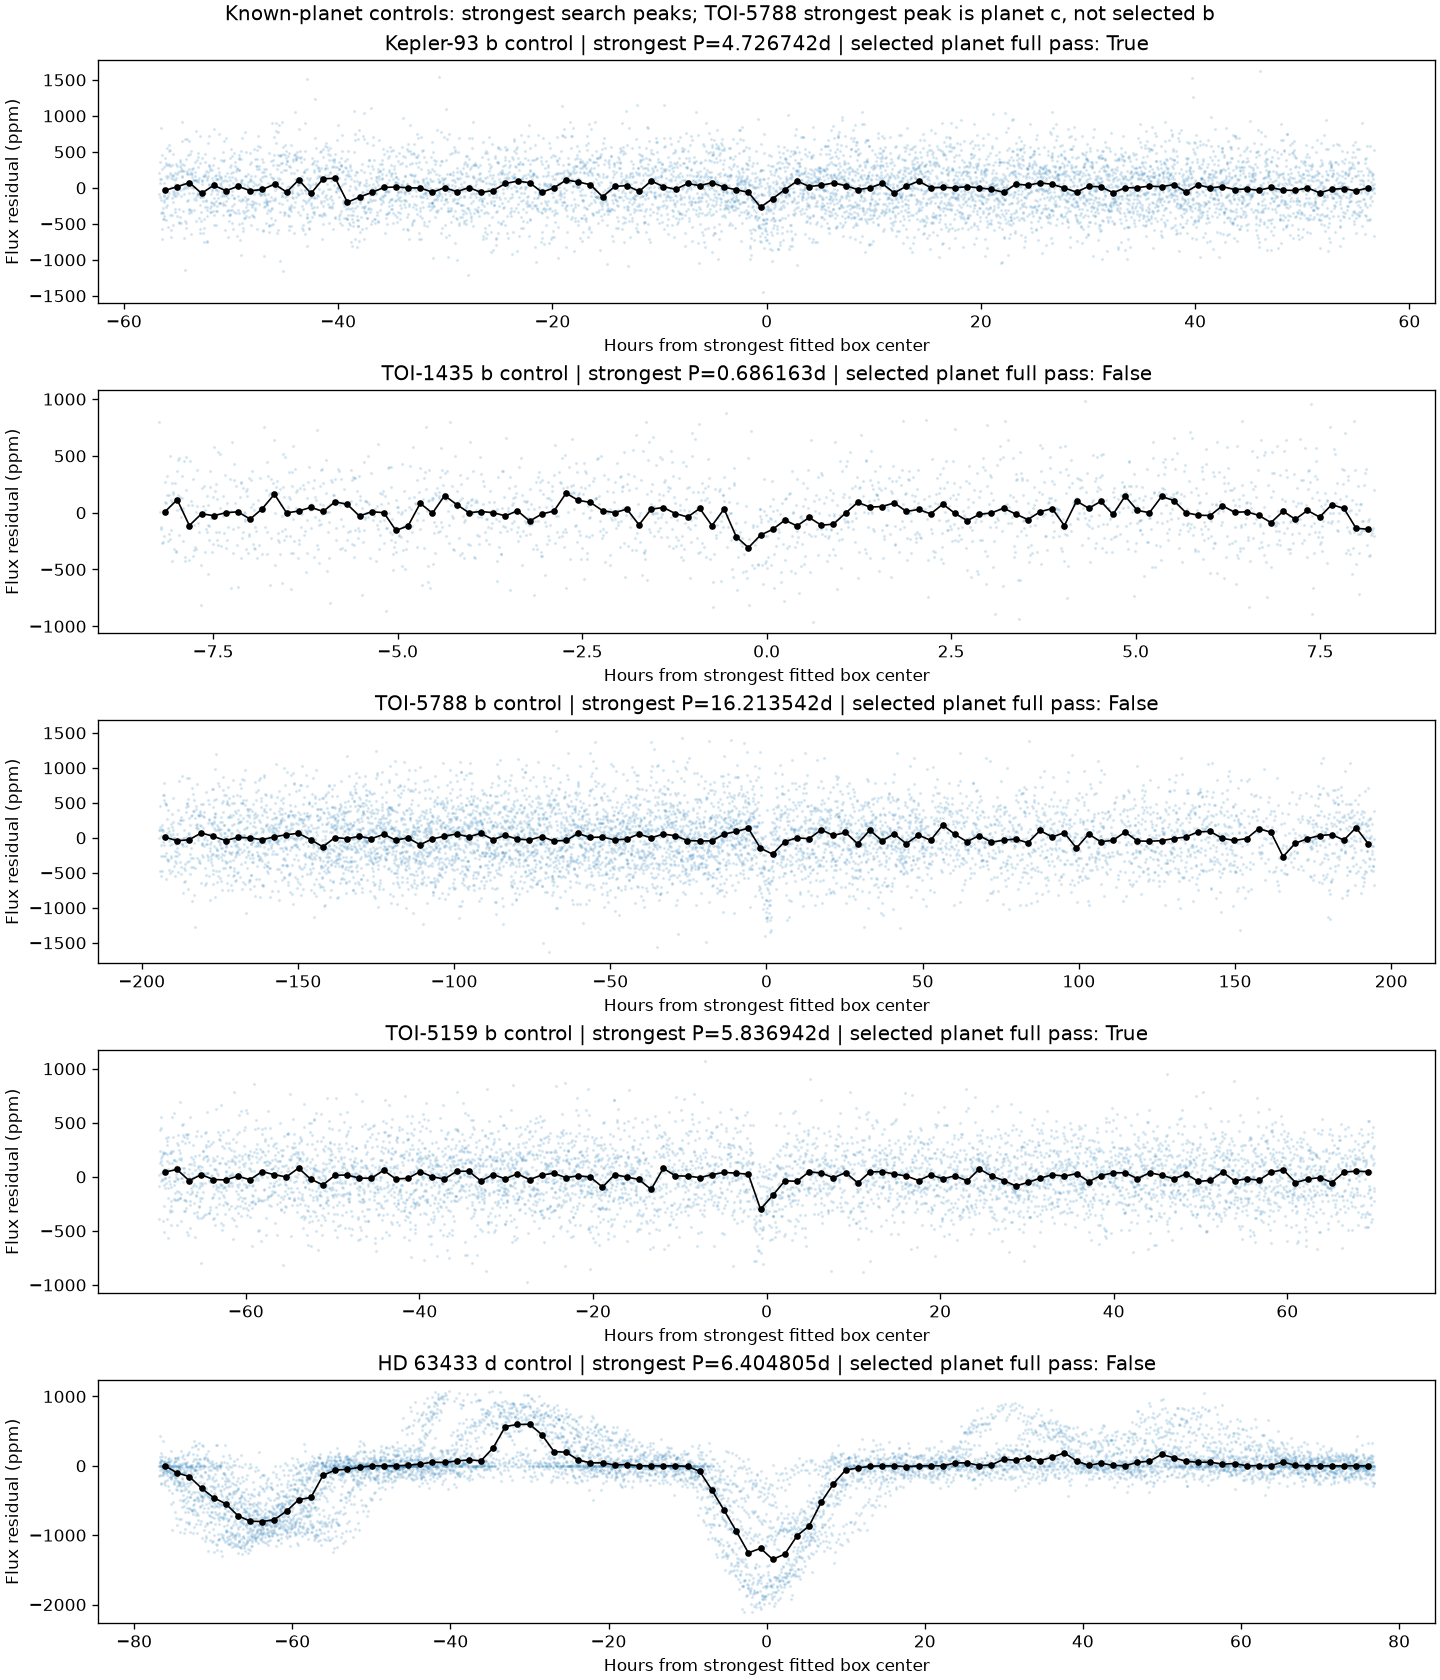
\includegraphics[width=\linewidth]{figures/controls-known.png}
\caption{Unchanged-pipeline searches of five preselected known planets.
The figure is retained from the archived control experiment. Successful
period agreement and full screening passage are different outcomes;
the two full passes do not establish population completeness.}
\label{fig:known-controls}
\end{figure}

The shallow-injection experiment applied exposure-integrated 100 and
300~ppm boxes to raw flux before detrending in three preselected
below-threshold targets. It tested periods 1.37, 4.73, and 13.13~days,
durations 0.04 and 0.12~days, and one phase per configuration.
All three 100-ppm recoveries occurred at the shortest period and longer
duration; none occurred at the two longer periods. Existing matching
baseline signals were not credited as recoveries. Thus negative searches
cannot exclude shallow planets on the basis of these examples.

For the two lower-priority signals in Table~\ref{tab:controls}, deterministic
0.25-, 0.5-, and 1-day blocks of paired raw flux and errors were permuted
within sector and gap-separated segments. Forty draws per model yielded
zero exceedances; each model's binomial 95\% Monte Carlo interval is
0--8.81\%. Counts were not pooled to claim a smaller bound.
Block seams, destroyed long correlations, retained signal fragments, and
unproven exchangeability limit interpretation. Four deterministic injections
for TIC 469309982 passed its local flag, but one selected a competing epoch
in one detrending; all four TIC 96166003 injections recovered the imposed
period and epoch. These checks verify processing behavior under selected
conditions, not the original search false-alarm probability.

\subsection{Attribution and uncertainty limitations}

Difference images compared mean local baseline and in-event pixels, with
propagated diagonal errors and inverse-variance event stacking. Conditional
source fits used mission response templates plus a planar background.
Neither fitted registration uncertainty nor response-model mismatch was
fully propagated into source rankings. Kepler-93~b exposes the practical
consequence: the target was preferred in sector 40, but a neighbor in
sector 41, despite a known shallow planetary signal. Stable rankings across
registration or event omissions can therefore accompany wrong attribution.

A separately frozen pointing-correction control passed three of four cases;
the contaminant's discrimination decreased in one sector. A template-free
paired-aperture diagnostic passed five of eight cases and preferred the wrong
Kepler-93 region twice. Neither met its gate for candidate application.
These failures prevent converting favorable candidate image fits into
calibrated host probabilities or using poor-model rankings alone to reject
a planet. Conditional circular, dark-occultor fits with exposure-integrated
\texttt{batman} models \cite{kreidberg2015} likewise assess compatibility
under assumed hosts and dilution; they do not exclude stellar companions.

Time-averaging audits of the two strongest signals follow the correlated-noise
rationale of \cite{pont2006}. They retain adverse event omissions and
insufficient-bin cases, but use different estimators: one compares fitted
residual bins with simulated white-noise refits, while the other examines
out-of-event bins. Their scalar error inflation is a sensitivity analysis,
not a complete covariance model or interchangeable reliability score.
Agreement between reductions sharing photons, successful arithmetic
verification, and conditional astrophysical scenario weights do not provide
independent observations or validation \cite{giacalone2021}.

\subsection{Detailed full-screen rejection gates}
\label{sec:screen-gates}

For reproducibility, a full-screen peak was flagged for any of the following:
formal SNR below 8; fewer than three supported events; an unmeasurable
odd/even comparison or discrepancy above $3\sigma$; an unmeasurable
half-phase secondary or secondary SNR above 3; inverted-to-original
maximum BLS power ratio at least 0.8; sinusoidal likelihood improvement
greater than the box improvement; or duty cycle $D/P>0.15$.
Additional flags applied when duration-binned correlated noise was
unmeasurable or reduced SNR below 7, event-depth consistency had conditional
chi-square survival below 0.001, one event contributed more than 75\%
of summed positive event SNR squared, or more than half the supported
events lay within $\max(0.15\,{\rm days},D)$ of a clean-segment edge.
The alternate detrending's strongest period had to agree within 2\%,
and every supplied aperture crowding fraction had to be at least 0.8.
Missing crowding information remained a flag, including for QLP products;
separately labeled diagnostic-only follow-ups did not erase original failures.
The discovery noise ratio used robust scatter of out-of-event duration-bin
means relative to their expected white errors, with a floor of one,
at least 15 bins, and at least half the expected sampling in each bin.
These exact numerical gates define the experiment; they do not constitute
an empirically calibrated planet classifier.

\clearpage
\section{The two priority signals}
\label{sec:primary}

\subsection{TIC 80387959: successful prediction tests with an unresolved host}

TIC 80387959 provides the clearest successful prediction test in this
investigation. Its adopted clock has period $P=4.192168718052227$ d,
reference midpoint $t_0=1575.375831123655$ BTJD, and fixed box duration
$D=0.092736$ d ($2.225664$ h). Throughout this paper,
$\mathrm{BTJD}=\mathrm{BJD}_{\mathrm{TDB}}-2457000$.
The digits specify the saved prediction; they do not imply that the physical
orbit is known to the displayed precision. Predictions based on the earlier
sectors were frozen before retrieval of QLP sectors 90 and 100. Without
adjusting the clock, the original follow-up procedure measured depths of
$621\pm98$ and $651\pm114$ ppm, respectively (Figure~\ref{fig:803holdout}).
Five and three events entered those measurements, of which four and two
passed the procedure's individual support criterion. The propagated timing
spreads, 0.02477 and 0.02679 d, were below the half-duration gate of
0.046368 d. These results support recurrence at the earlier prediction,
while leaving the variable source and physical explanation undetermined.

\begin{figure}[tbp]
\centering
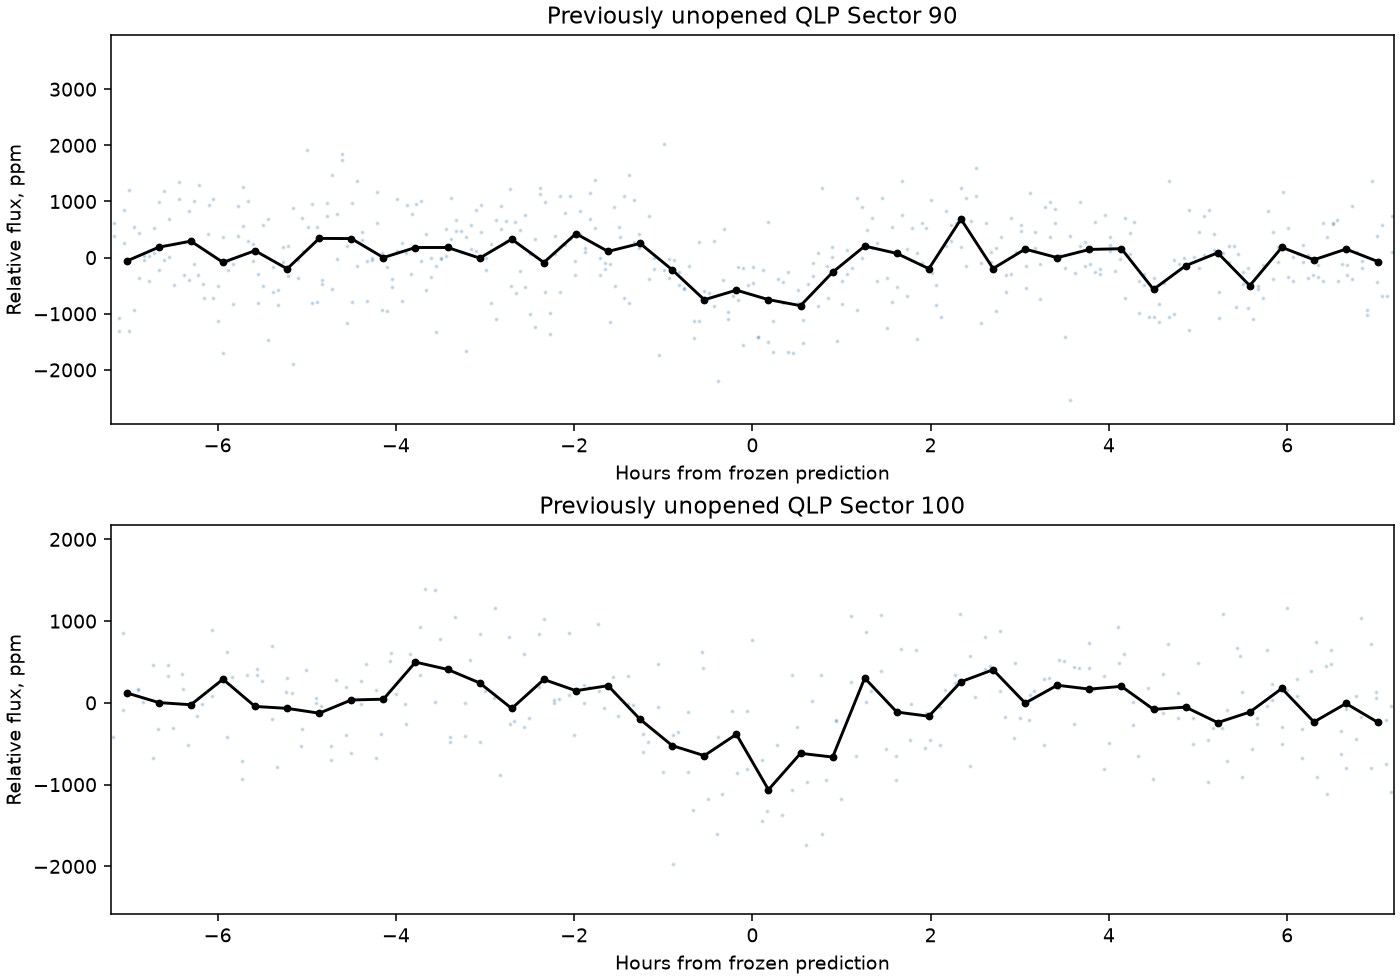
\includegraphics[width=0.96\linewidth]{figures/803-holdout.png}
\caption{TIC 80387959 in QLP sectors 90 and 100 at the prediction fixed
before those products were retrieved. These are the original follow-up
reductions, with their original preprocessing and sampling. Positive
recurrence at the fixed clock is evidence about the signal; it does not
identify the star producing it. Displayed measurement errors are
conditional on the adopted processing and noise model.}
\label{fig:803holdout}
\end{figure}

A subsequent retrospective test used native corrected flux from all six
already inspected sectors, without an additional global flattening filter.
It fitted an exposure-integrated box simultaneously with separate local
intercepts and slopes for each event. Table~\ref{tab:803depths} reports these
measurements, which have different samples and nuisance models from the
original prediction test. All six sectors and every single-event omission
retain a positive depth; the smallest omitted-event depth is 494 ppm in
sector 100. Thirty event windows enter this particular analysis.
Neither these windows nor alternative reductions of their exposures are
thirty independent confirmations of a planetary interpretation.

\begin{table}[tbp]
\centering
\caption{TIC 80387959: retrospective joint local-baseline box fits.
The final column applies a heuristic time-averaging noise inflation to the
same depth estimates. All errors are conditional, not complete uncertainty
budgets or calibrated search significances.}
\label{tab:803depths}
\begin{tabular}{rlrrr}
\toprule
Sector & Product & Events & Depth (ppm) & Adjusted error (ppm) \\
\midrule
10  & TESS-SPOC PDCSAP & 4 & $1038\pm109$ & 113 \\
36  & TESS-SPOC PDCSAP & 6 & $813\pm87$   & 92 \\
37  & TESS-SPOC PDCSAP & 5 & $904\pm91$   & 105 \\
63  & TESS-SPOC PDCSAP & 5 & $807\pm93$   & 130 \\
90  & QLP DET\_FLUX   & 6 & $613\pm89$   & 92 \\
100 & QLP DET\_FLUX   & 4 & $582\pm99$   & 133 \\
\bottomrule
\end{tabular}
\end{table}

\begin{figure}[tbp]
\centering
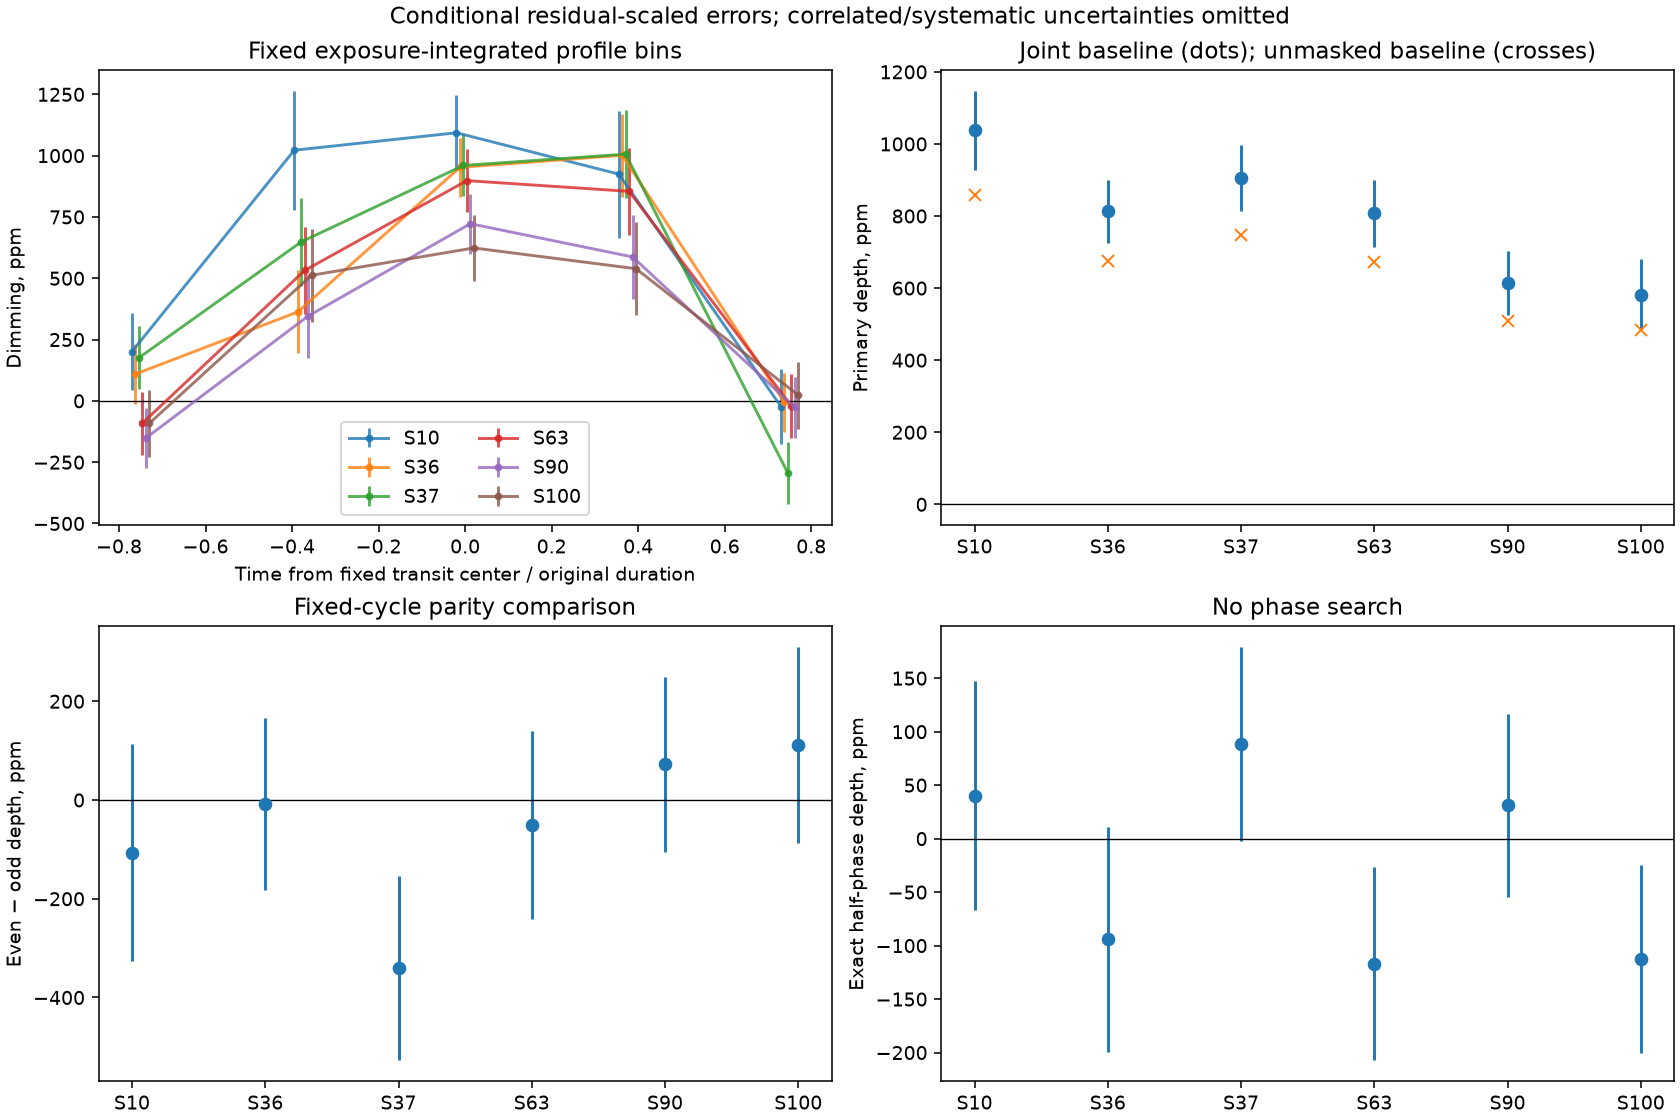
\includegraphics[width=0.97\linewidth]{figures/803-shape.png}
\caption{Six-sector fixed-clock shape, depth, parity, and half-phase tests
for TIC 80387959. Native corrected-flux models jointly fit local event
baselines, without additional global flattening. All data were already
inspected before this retrospective analysis. Conditional errors omit a
complete correlated-noise and dilution model. A positive dip across these
tests does not exclude a blended stellar eclipse.}
\label{fig:803shape}
\end{figure}

No coherent odd/even difference or secondary eclipse exactly half a cycle
away emerges (Figure~\ref{fig:803shape}). An isolated sector-36
ingress-minus-egress contrast of $-639\pm233$ ppm is retained rather than
interpreted as a replicated asymmetry. A secondary at another phase,
strong dilution, or an unresolved companion could evade these checks.
The descriptive depth means differ between the four older TESS-SPOC
sectors ($877\pm47$ ppm) and the later QLP sectors ($599\pm66$ ppm).
This is not established physical depth evolution. Same-epoch paired
products give SPOC-minus-QLP differences of $+47\pm76$ ppm in sector 36
and $-163\pm96$ ppm in sector 37, offering no consistent pipeline offset.
Common-quality sampling itself changes fitted depths, and the later
QLP extraction changed beginning in sector 94 \cite{petitpas2026}.

Time-averaging diagnostics motivated by \cite{pont2006} increase the
sector-100 error from 99 to 133 ppm. Its worst event-omission depth/error
ratio is 2.96. These checks weaken the apparent precision without removing
the signal; they do not calibrate its false-alarm probability. Four-sector
orbital-harmonic tests likewise find no stable substantial modulation, but
pipeline correction can suppress broad variability and this null result
cannot exclude binaries.

Independent survey context is modestly favorable for the bright star.
One securely associated RAVE observation on 2010 May 2 gives
$5.94\pm0.87$ km s$^{-1}$, consistent with the Gaia aggregate velocity
$7.02097\pm0.32064$ km s$^{-1}$ at 1.17 combined formal error units.
Predominantly normal RAVE morphology and dwarf-like atmospheric parameters
do not constitute a companion exclusion. There is only one RAVE epoch,
the surveys have different systematics, and a faint eclipsing neighbor
would not be tested by this agreement. Gaia's available RV diagnostics
provide no strong variability flag, but no orbital sensitivity or mass
limit has been established.

\subsection{TIC 402358350: localized recurrence with a failed timing gate}

For TIC 402358350, the expanded clock frozen before sector 81 has
$P=11.769544332077816$ d, $t_0=2392.9928689397047$ BTJD, and
$D=0.144$ d ($3.456$ h). It incorporated sectors 40, 41, and 54;
sector 54 had already been examined and is not an independent test of this
expanded model. The original discovery clock was different and is retained
in the evidence record.

The primary sector-81 prediction yields $634.6\pm72.2$ ppm with two
supported events. However, its timing-profile spread of 0.09142 d exceeds
the predeclared $D/2=0.072$ d gate. Consequently this is a positive dimming
measurement with \emph{inconclusive prediction timing}, despite a formal
depth/error ratio of 8.79. The alternate expanded reduction and both
original-clock reductions also fail timing precision. All four comparisons
are shown in Figure~\ref{fig:402holdout}; selecting the deepest comparison
would not repair this failure.

\begin{figure}[tbp]
\centering
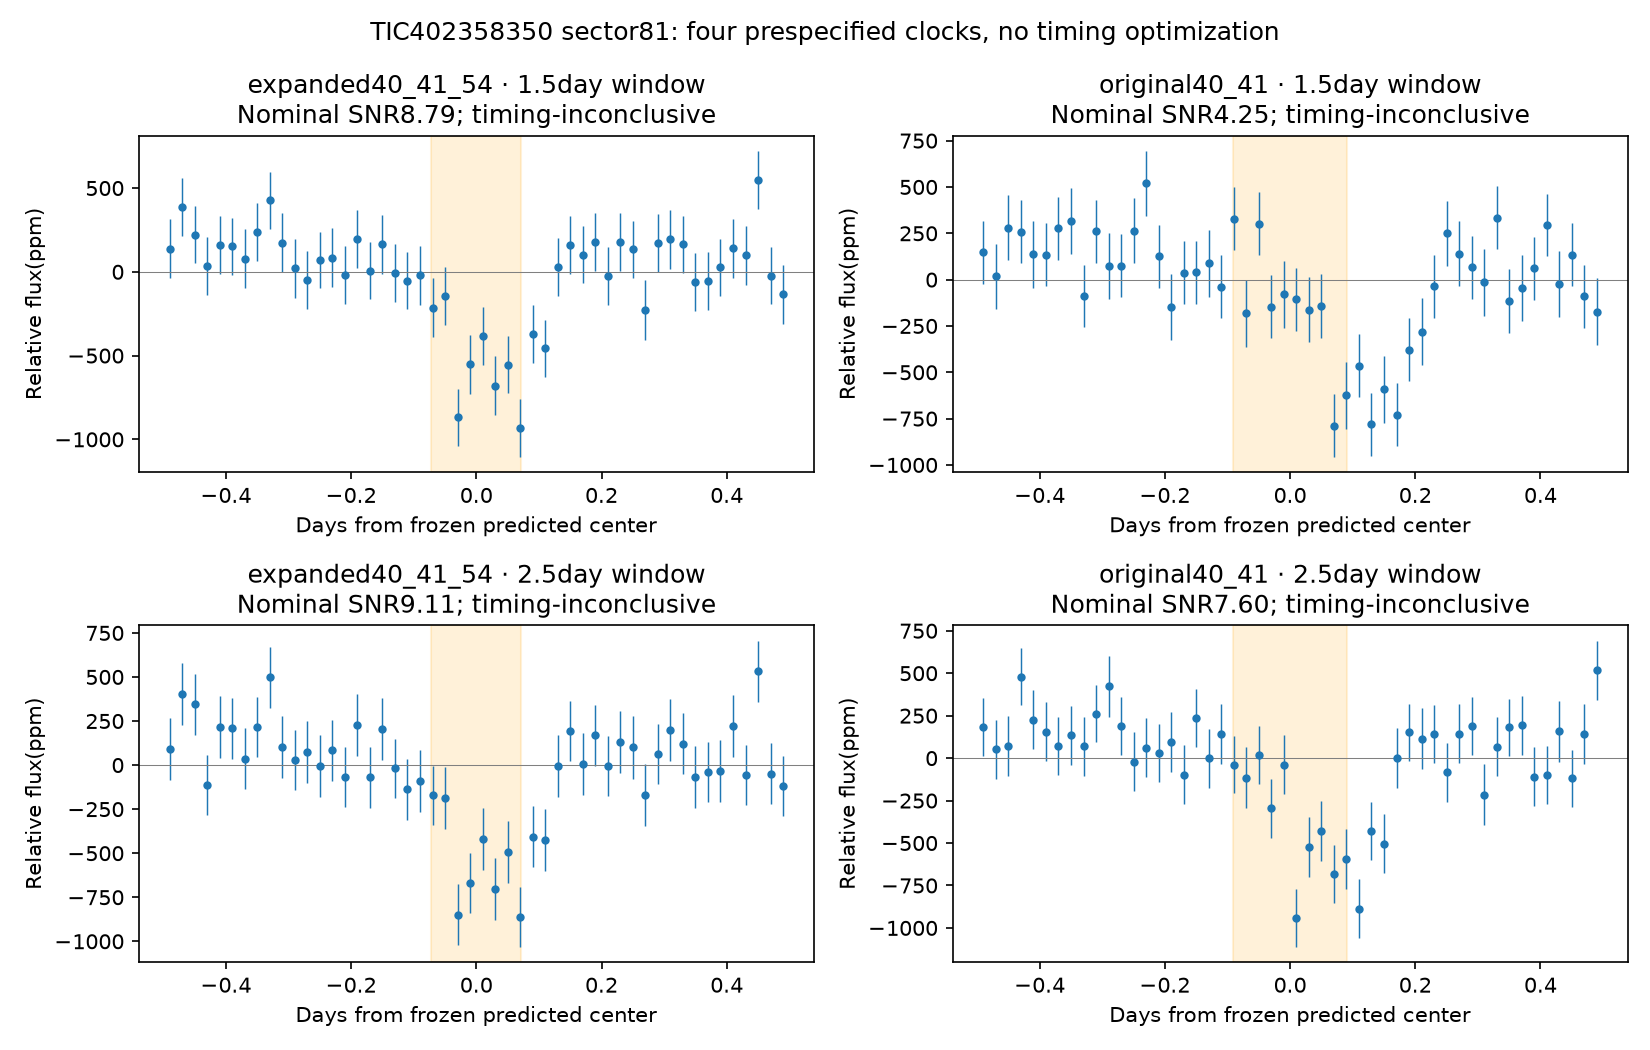
\includegraphics[width=0.96\linewidth]{figures/402-holdout.png}
\caption{Sector-81 measurements for all four predictions fixed before
access to TIC 402358350's sector-81 photometry. The expanded primary clock
places a compact dip near the predicted center, but its timing spread
exceeds the unchanged precision gate. The comparisons share the same
sector-81 photons; neither alternate preprocessing nor a positive formal
depth converts the result into a passed timing test.}
\label{fig:402holdout}
\end{figure}

A separate retrospective test directly fitted native SAP and PDCSAP
photometry, normalized by each sector's median. Polynomial baselines of
degree zero, one, and two used points outside the protected interval
$|t-t_c|\leq D$, with outer radii $3D$ or $5D$. No running-median
flattening or data-dependent clipping was added. Nine nominal centers fall
within the sector spans; one sector-40 event lies in a gap and fails
coverage for all twelve methods. The remaining eight events are positive
under every method, yielding the 590--659 ppm combined depths in
Table~\ref{tab:402baseline}. Leaving out any one event retains
569--706 ppm across the matrix. Thus no individual dip or single baseline
choice creates the measured recurrence.

\begin{table}[tbp]
\centering
\caption{TIC 402358350: the complete twelve-method baseline matrix.
Errors include baseline extrapolation uncertainty and residual-scatter
scaling; correlations and source uncertainty remain incompletely modeled.
SAP and PDCSAP are reductions of the same exposures.}
\label{tab:402baseline}
\begin{tabular}{llrr}
\toprule
Baseline & Outer radius & SAP depth (ppm) & PDCSAP depth (ppm) \\
\midrule
Constant  & $3D$ & $627\pm44$ & $609\pm42$ \\
Constant  & $5D$ & $602\pm41$ & $591\pm40$ \\
Linear    & $3D$ & $642\pm41$ & $610\pm42$ \\
Linear    & $5D$ & $614\pm39$ & $590\pm39$ \\
Quadratic & $3D$ & $659\pm53$ & $647\pm54$ \\
Quadratic & $5D$ & $633\pm43$ & $621\pm43$ \\
\bottomrule
\end{tabular}
\end{table}

\begin{figure}[tbp]
\centering
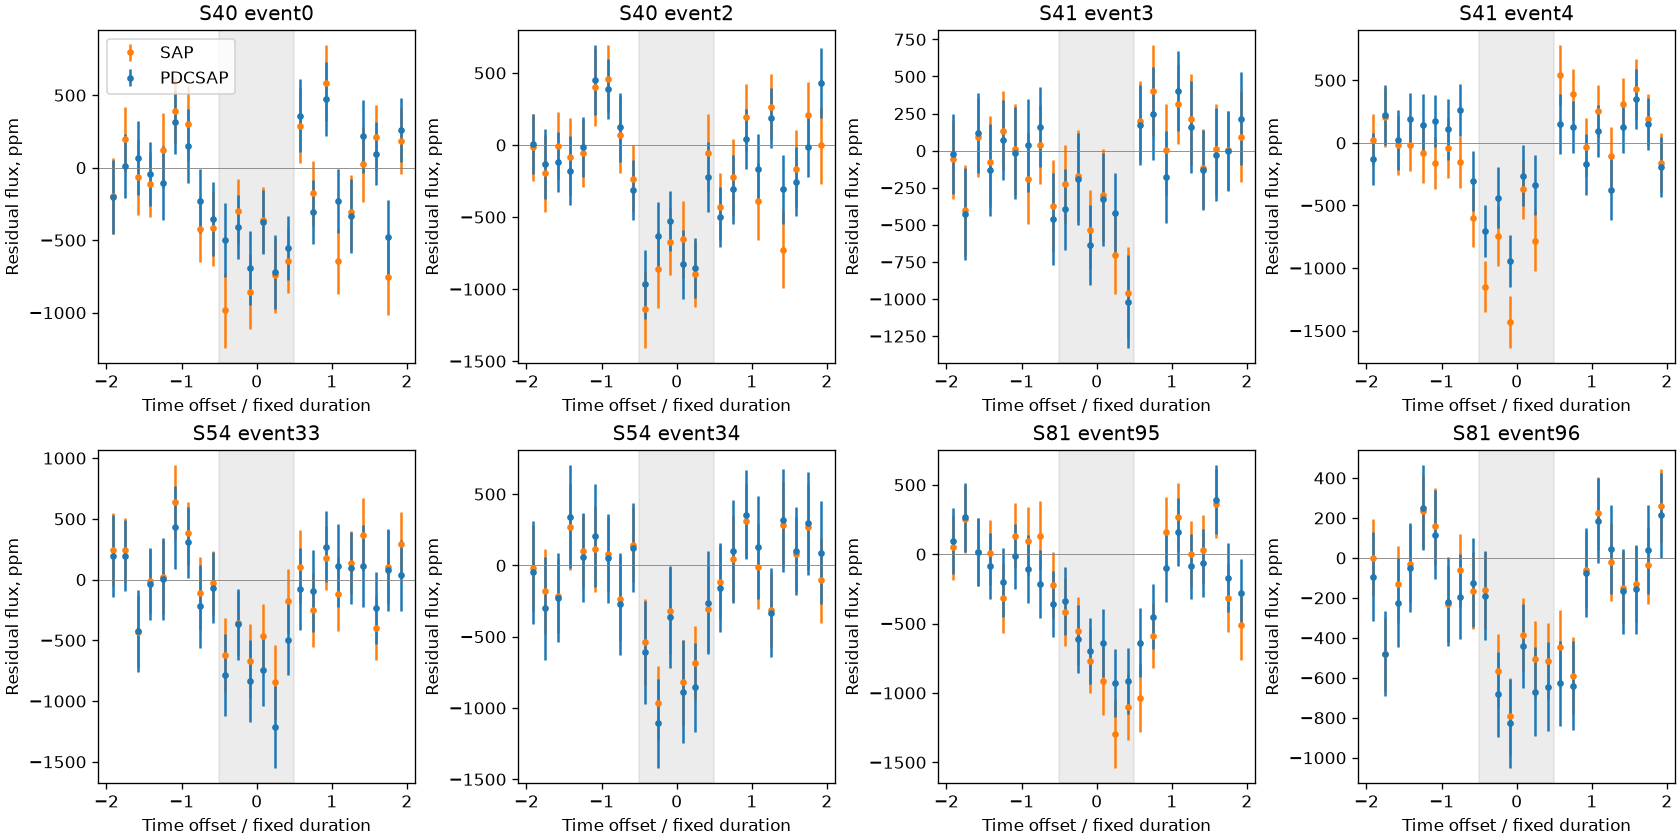
\includegraphics[width=0.98\linewidth]{figures/402-events.png}
\caption{All eight usable TIC 402358350 events, illustrated with the
linear-$3D$ baseline specified in the method matrix. SAP and PDCSAP retain
positive dips and share photons. The protected event intervals and local
baselines test whether additional global smoothing created the feature;
they do not establish the host. Errors follow the conditional measurement
model and do not include all timing or instrumental uncertainty.}
\label{fig:402events}
\end{figure}

\begin{figure}[tbp]
\centering
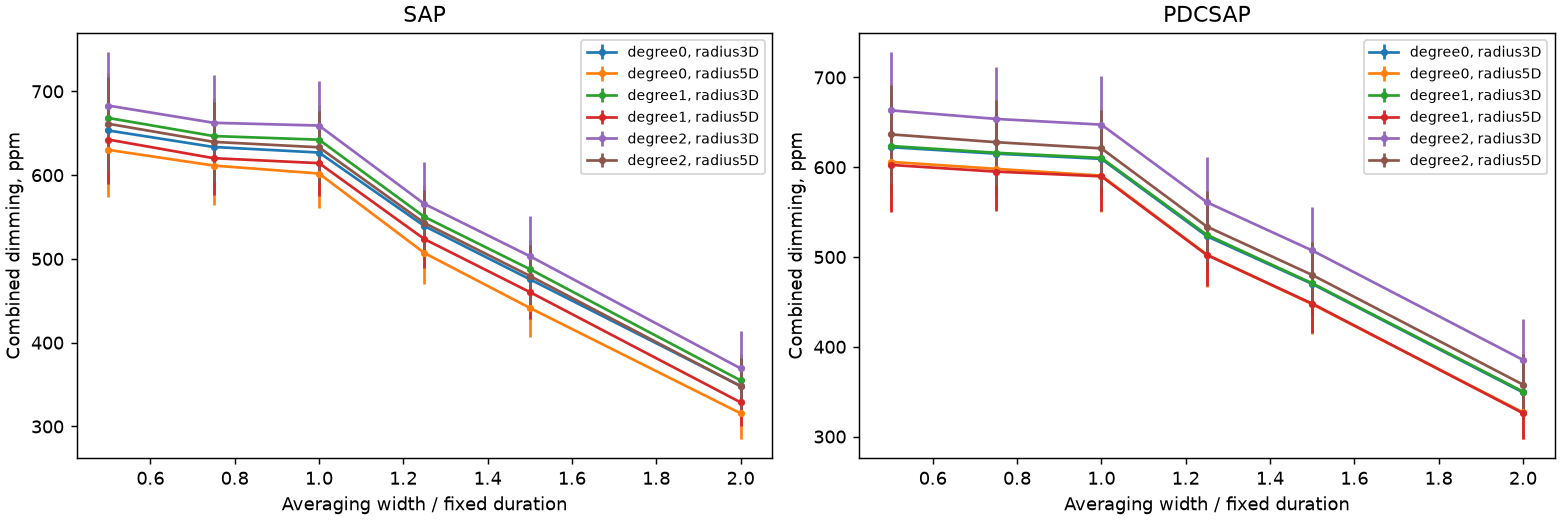
\includegraphics[width=0.96\linewidth]{figures/402-widths.png}
\caption{TIC 402358350's retained averaging-width and baseline matrix.
Central depths are approximately stable between widths $0.5D$ and $D$,
and decrease as wider windows include the shoulders. This supports
localization in time; the displayed widths are fixed diagnostic choices,
not a fitted transit-duration posterior. Rows and columns reuse the same
events and are not independent trials.}
\label{fig:402widths}
\end{figure}

The width tests show a localized depression rather than a uniformly broad
low state (Figure~\ref{fig:402widths}). Adverse controls remain material:
one matched SAP offset window is deeper than its associated event under
five of six baselines, and a sector-54 event has no matched controls.
Time-averaging inflation expands combined errors to 41--93 ppm, depending
on baseline; linear-$3D$ results change only to $642\pm43$ and
$610\pm44$ ppm. Scalar inflation is a sensitivity diagnostic rather than
a full noise likelihood.

The nearby published pulsator TIC 402358249 has dominant frequency
0.9517724 d$^{-1}$ (period 1.050671358 d). Adding sine and cosine nuisance
terms at this fixed frequency leaves SAP depths near 578 ppm and PDCSAP
depths near 610--621 ppm. This rules out only that simple sinusoidal model
as a complete explanation. Conversely, deterministic 1000-ppm sinusoidal
injections into the archived products can shift a sector's box depth by
up to 1209 ppm after sampling and flattening
(Figure~\ref{fig:pulsator}). Smooth variability can therefore couple
strongly into these measurements; the experiment neither bounds the real
contamination nor reruns the upstream telescope reduction.

\begin{figure}[tbp]
\centering
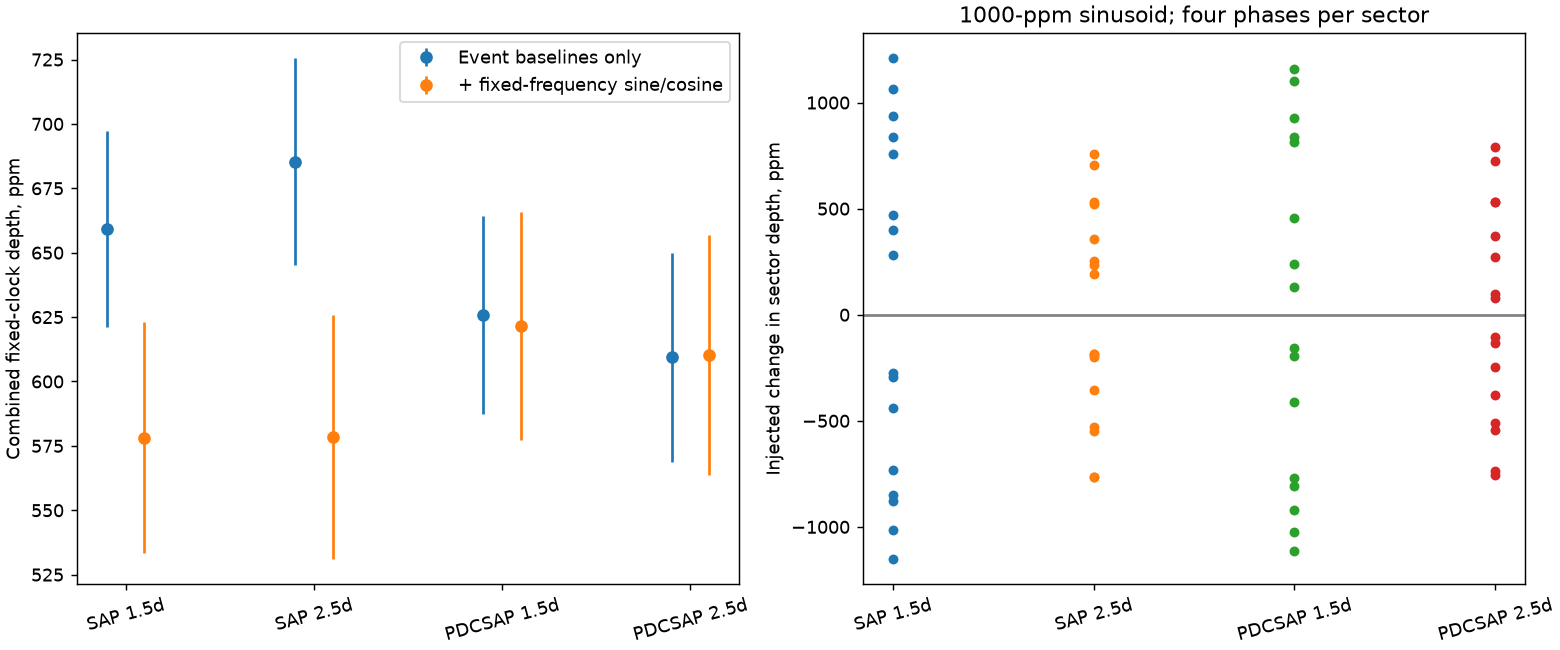
\includegraphics[width=0.96\linewidth]{figures/pulsator-tests.png}
\caption{TIC 402358350's fixed-frequency pulsation nuisance fits and
deterministic sinusoid-transfer tests. The nuisance sinusoid does not
absorb the recurring dip, while the injection response demonstrates
substantial sampling and preprocessing sensitivity. These are
retrospective tests of already inspected products, not independent
observations, an astrophysical contamination model, or a false-alarm
calibration.}
\label{fig:pulsator}
\end{figure}

\section{Source attribution and competing stellar hosts}
\label{sec:host}

Repeatable dimming and identification of its host are separate requirements.
For TIC 80387959, stacked image models prefer the target in sectors 36,
37, and 100, TIC 80387965 in sector 63, and TIC 80387961 in sector 90.
Every sector changes its preferred host under at least one event omission
(Figure~\ref{fig:hostinstability}). For TIC 402358350, the discovery
sectors disagree, while later whole-stamp fits favor the target region
with substantial structured residuals and sensitivity to the fitted image
region. A known shallow planet, Kepler-93 b, is incorrectly assigned a
neighbor preference by this same procedure in one tested sector.
Consequently model rankings, even stable ones, are not calibrated host
probabilities or sufficient planet vetoes.

\begin{figure}[tbp]
\centering
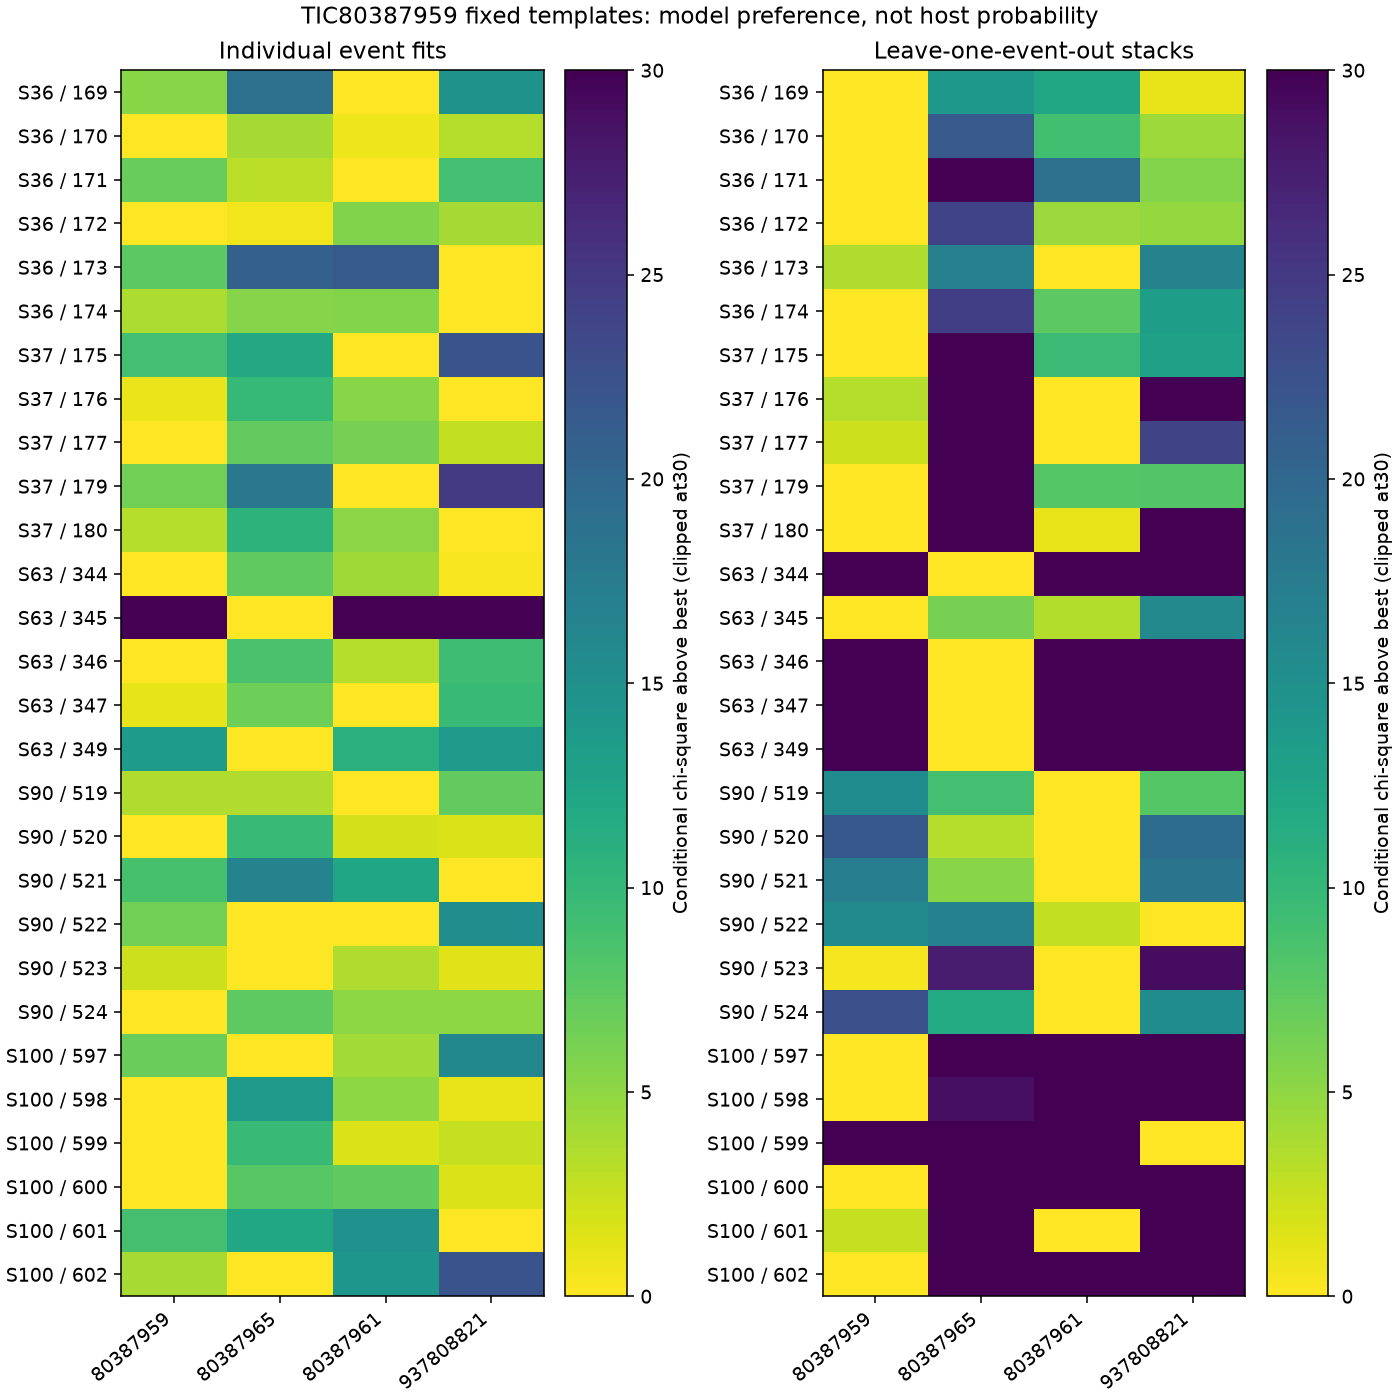
\includegraphics[width=0.96\linewidth]{figures/host-instability.png}
\caption{Event-level and omission sensitivity of TIC 80387959's source
rankings. Different sectors and subsets prefer different stars.
Overlapping omissions are correlated diagnostics. Inadequate image
residuals and a failed known-host control prevent interpreting the
chi-square rankings as probabilities or selecting target-favoring subsets
as definitive source attribution.}
\label{fig:hostinstability}
\end{figure}

The aperture-light budget supplies a complementary constraint
\cite{giacalone2022}. If a neighbor contributes a fraction $f$ of the
aperture light, its intrinsic eclipse must have depth $e=d/f$ to produce
an observed SAP decrement $d$. Under equal target/neighbor throughput,
TIC 80387965, 13.76 arcsec away, needs approximately 1.41--1.72\%
eclipses; TIC 80387961, 7.54 arcsec away, needs 24.19--29.47\%.
For TIC 402358350, TIC 1918682563 at 10.12 arcsec needs
24.76--28.86\%. These are conditional requirements, not observed
eclipses. Some fainter competitors exceed 100\% under nominal assumptions,
but uncertain response, catalog identity, magnitude, and depth reopen them
in the declared sensitivity tests (Figure~\ref{fig:eclipsebudget}). No
listed close competitor is safely excluded, and unresolved companions
are unconstrained by this resolved-source budget.

\begin{figure}[tbp]
\centering
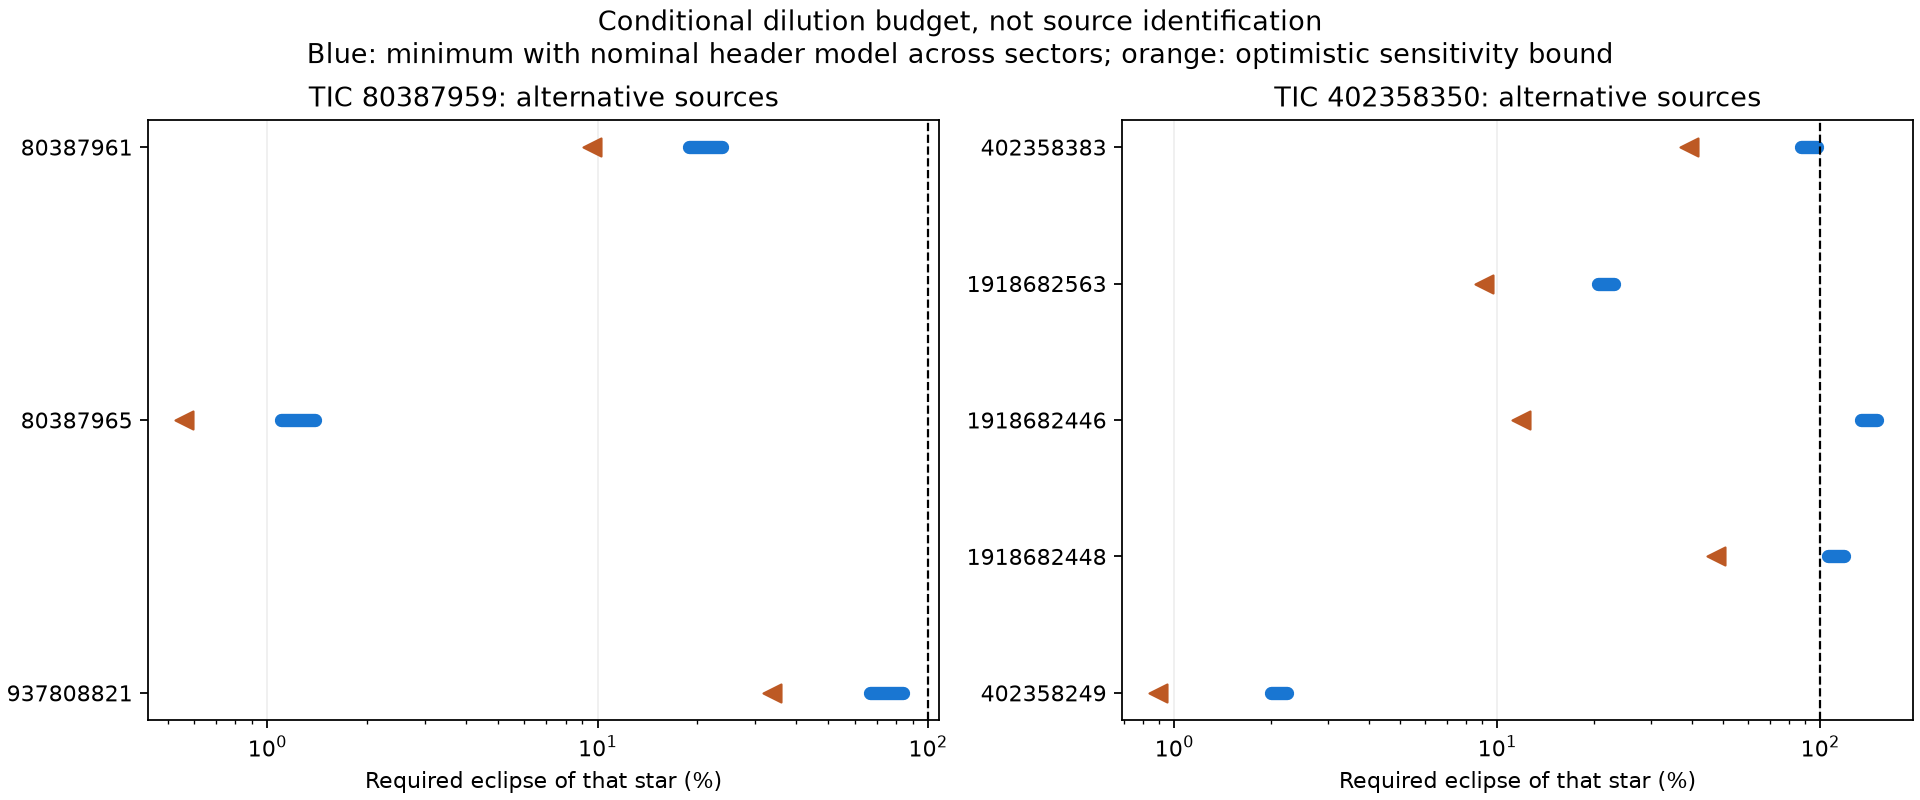
\includegraphics[width=0.97\linewidth]{figures/host-eclipses.png}
\caption{Conditional intrinsic eclipses required on nearby sources.
Requirements use native SAP decrements and alternative aperture-response
assumptions. Pipeline crowding and captured-flux estimates are models,
not independent response measurements. The optimistic cases are declared
stress tests rather than confidence limits. A nominal requirement above
100\% does not exclude a source whose catalog or throughput model is
uncertain.}
\label{fig:eclipsebudget}
\end{figure}

Resolved archival photometry has not closed this gap. For TIC 80387968,
35.34 arcsec from TIC 80387959, 43 quality-selected SkyMapper measurements
include two differently colored samples during one predicted event, with
no dimming. They disfavor a particular same-depth, flat-bottom eclipse at
those instants, but fail the predeclared two-event exclusion gate.
Color, eclipse shape, and calibration remain limitations. Around
TIC 402358350, four ZTF streams for TIC 1918682563 retain 288 accepted
measurements with large scatter; all 48 fixed-clock comparisons are
inconclusive. A separate six-stream test of TIC 74037550 retains 545
measurements and all 72 comparisons are inconclusive. Sparse sampling and
propagated timing uncertainty prevent eclipse exclusions, even where
nominal precision would otherwise appear sufficient.

\section{Conditional astrophysical scenario calculations}
\label{sec:models}

We used TRICERATOPS 1.1.0 \cite{giacalone2021} as an exploratory comparison
of astrophysical scenarios, applying it to one already examined sector per
target: sector 36 for TIC 80387959 and sector 54 for TIC 402358350.
The native SAP inputs remove previously fitted event baselines, retaining
482 samples from six events and 230 samples from two events, respectively.
The calculations use the diluted-flux convention and explicit exposure
integration. Baseline covariance is not marginalized, stellar parameters
are held fixed, and a nominal Gaussian aperture response controls nearby
host eligibility. Verified exact catalog duplicates were removed while
preserving the superseded inputs and calculations.

All 17 bounded runs and three provenance replays were completed. The
nominal set contains three 100,000-draw seeds and one million-draw seed
per target; the remaining runs test noise sensitivity and diagnostic
controls. Table~\ref{tab:triceratops} gives the million-draw values.
The original requirement of three independent million-draw calculations
per target was not met, so convergence is unestablished. Three smaller
seeds span 92.2334--92.7963\% and 97.3632--97.8000\% in target-primary
weight; these ranges measure numerical scatter rather than physical
uncertainty (Figure~\ref{fig:triceratops}).

\begin{table}[tbp]
\centering
\caption{Single-seed, million-draw TRICERATOPS scenario weights.
These are conditional on the supplied single-sector data and modeled
scenarios; neither target passes the joint numerical validation thresholds.}
\label{tab:triceratops}
\begin{tabular}{lrrr}
\toprule
TIC & Target-primary planet weight & FPP & NFPP \\
\midrule
80387959  & 92.4284\% & 7.5716\% & 4.2862\% \\
402358350 & 97.6834\% & 2.3166\% & 0.3959\% \\
\bottomrule
\end{tabular}
\end{table}

\begin{figure}[tbp]
\centering
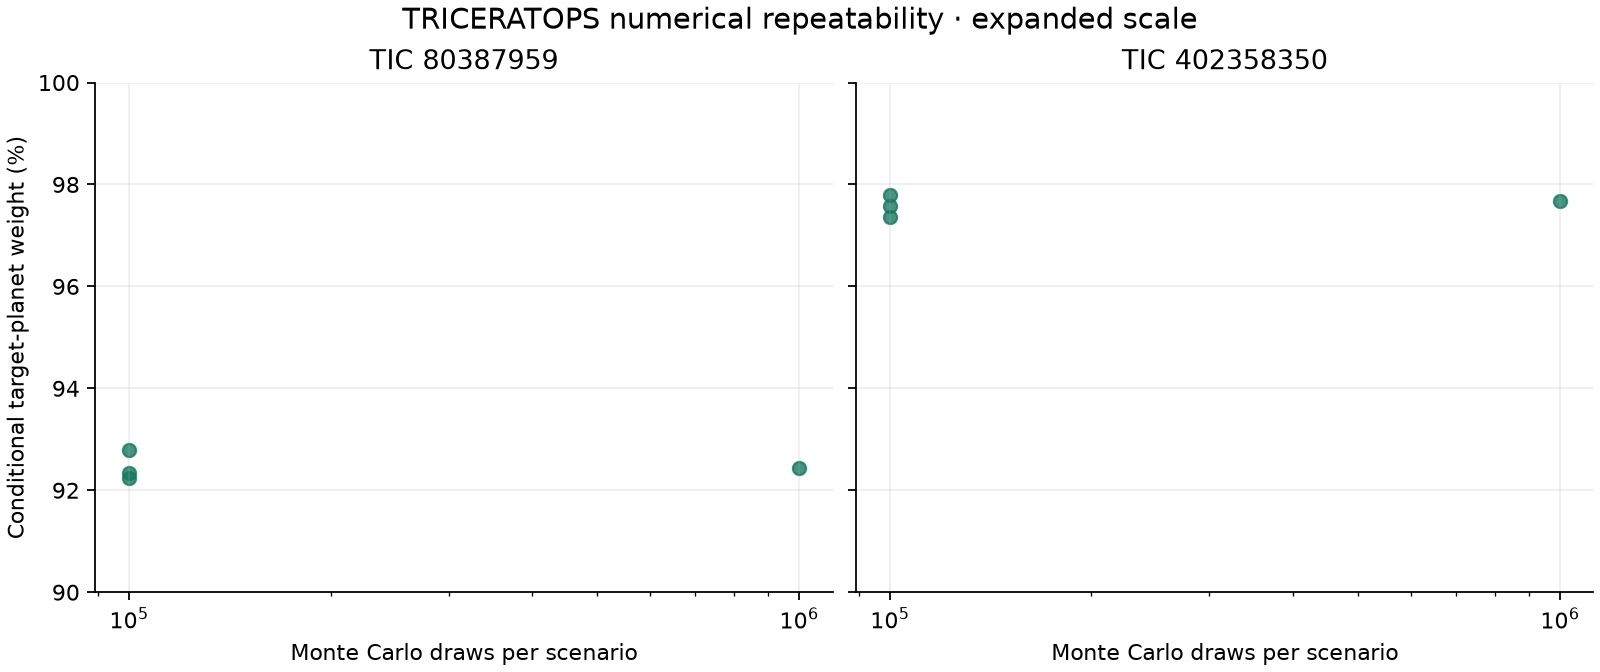
\includegraphics[width=0.96\linewidth]{figures/triceratops-convergence.png}
\caption{Adopted nominal TRICERATOPS runs at two draw counts.
Repeated smaller calculations test Monte Carlo sensitivity, but one
million-draw seed per target leaves the original convergence criterion
unmet. The scenario weights exclude general artifacts and stellar
variability, and do not quantify discovery reliability. The two targets
also retain different observational timing and attribution limitations.}
\label{fig:triceratops}
\end{figure}

Here $1-\mathrm{FPP}$ sums planet scenarios around the target primary,
including the package's dilution alternatives. FPP includes some planets
on other stars; NFPP includes all resolved-neighbor scenarios, including
neighboring planets. Neither candidate meets both published numerical
criteria, $\mathrm{FPP}<0.015$ and $\mathrm{NFPP}<0.001$; both also fail
the nearby-source threshold for the method's less restrictive
``likely planet'' category. These thresholds do not independently transfer
the calibration of the published workflow to the present exploratory inputs.

The omitted-model problem is visible in controls. Setting the flux
identically to unity still yields target-primary planet weights of
44.15\% and 23.38\%; inverted signals yield 41.99\% and 15.91\%.
These tests retain the supplied clock and observed-depth host eligibility,
so they are computational diagnostics, not false-alarm experiments.
Doubling the scalar noise changes nominal weights to 91.98\% and 93.74\%.
The restricted Kepler-93 b control returns 82.88\% and fails the validation
thresholds despite that planet's independent establishment. The scenario
family lacks general instrumental and stochastic stellar-variability
alternatives and normalizes its weights even for unconvincing inputs.
Accordingly these percentages do not measure the probability of a real
planet or a new discovery. TIC 402358350's larger weight does not repair
its timing failure or make its overall evidence stronger than that for
TIC 80387959.

\clearpage
\section{Four additional signals and their limitations}
\label{sec:other}

The remaining four signals illustrate distinct obstacles: a deep event with
ambiguous companion size, two shallow signals with inadequate predictive timing,
and recurring dimming for which a resolved neighboring binary is a plausible
source. All measurements below retain the historical clocks and unfavorable
alternatives. Formal errors describe the stated measurement model; they omit
some correlated noise, timing and source uncertainties. Repeated reductions of
one sector do not constitute independent observations.

\subsection{TIC 241928959: target-region dimming with physical degeneracies}
\label{sec:tic241}
% Evidence: results/qlp-faint-midradius-single-review-20261011/241928959-peak0/ASSESSMENT.md
% results/event-baseline-six-20261012/ASSESSMENT.md

The approximately 3.533-day pattern is measured in sector 92 alone. Its refined
training clock is $P=3.532592898$~d with a 0.032-day box duration. Five usable,
discovery-selected events give an event-baseline depth of $11\,992\pm786$~ppm;
removing each event in turn leaves $11\,729$--$12\,442$~ppm. One disturbed event
remains excluded because its in-window samples carry nonzero quality flags and
lack a usable baseline. The 2.5-day detrending removes another event's
in-transit samples, leaving four observed transits. The physical fitter's six
local windows include baseline-only windows and must not be counted as six
transits. The deeper final event remains in the analysis.

% Evidence: results/prf-fullscene-241928959-20261011/ASSESSMENT.md
% results/prf-events-241928959-20261011/ASSESSMENT.md
Difference images favor the target region over TIC 241928961, a neighbor
10.56~arcsec away. A fuller scene model gives $\chi^2=109.16$ for the target
and 437.05 for that neighbor, each with 117 degrees of freedom. All five
individual events and their omission stacks prefer the target in the original
brighter-scene model. These conditional template comparisons do not exclude
unresolved companions or calibrate host probabilities. An illustrative
equal-throughput blend with the known neighbor would require a roughly
24\% eclipse; the actual aperture response is not known.

% Evidence: results/physical-241928959-20261012/ASSESSMENT.md
The short shape does not provide a secure companion radius
(Figure~\ref{fig:241physical}). For the 1.5-day reduction, a circular,
undiluted target model with freely fitted $a/R_\star$ gives radius ratio
$k=0.1257$, impact parameter $b=0.840$ and an inferred stellar density
$15.66~\mathrm{g\,cm^{-3}}$. The nominal catalog mass and radius imply only
about $3.21~\mathrm{g\,cm^{-3}}$. A broad prior on $a/R_\star$ instead permits
$k=0.3072$ and $b=1.135$, a grazing configuration, at a data-fit cost of only
$\Delta\chi^2\simeq1.7$. The second detrending retains this degeneracy.
Eccentricity, dilution and stellar-model errors remain unmodeled alternatives.
The restricted neighbor fit reaches its upper radius-ratio bound; it is not a
general eclipsing-binary exclusion.

% Evidence: results/companion-constraints-shortlist-20261012/ASSESSMENT.md
% results/parity-241928959-20261011/ASSESSMENT.md
% results/secondary-241928959-20261011/ASSESSMENT.md
% results/coverage-review-241928959-20261011/ASSESSMENT.md
Gaia RUWE 3.356 and a 14\% multiple-peak image fraction reinforce caution about
a single-star interpretation, without demonstrating a companion. Alternating
depths differ by less than one formal standard deviation, but only one usable
odd-family event is available. Fixed half-phase tests find no convincing
secondary eclipse and do not exclude an eccentric or faint binary. Existing
ZTF measurements are inconclusive, and the checked TESS coverage supplies no
verified second observing epoch. Source identity, companion size and recurrence
therefore remain unresolved.

\begin{figure}[p]
\centering
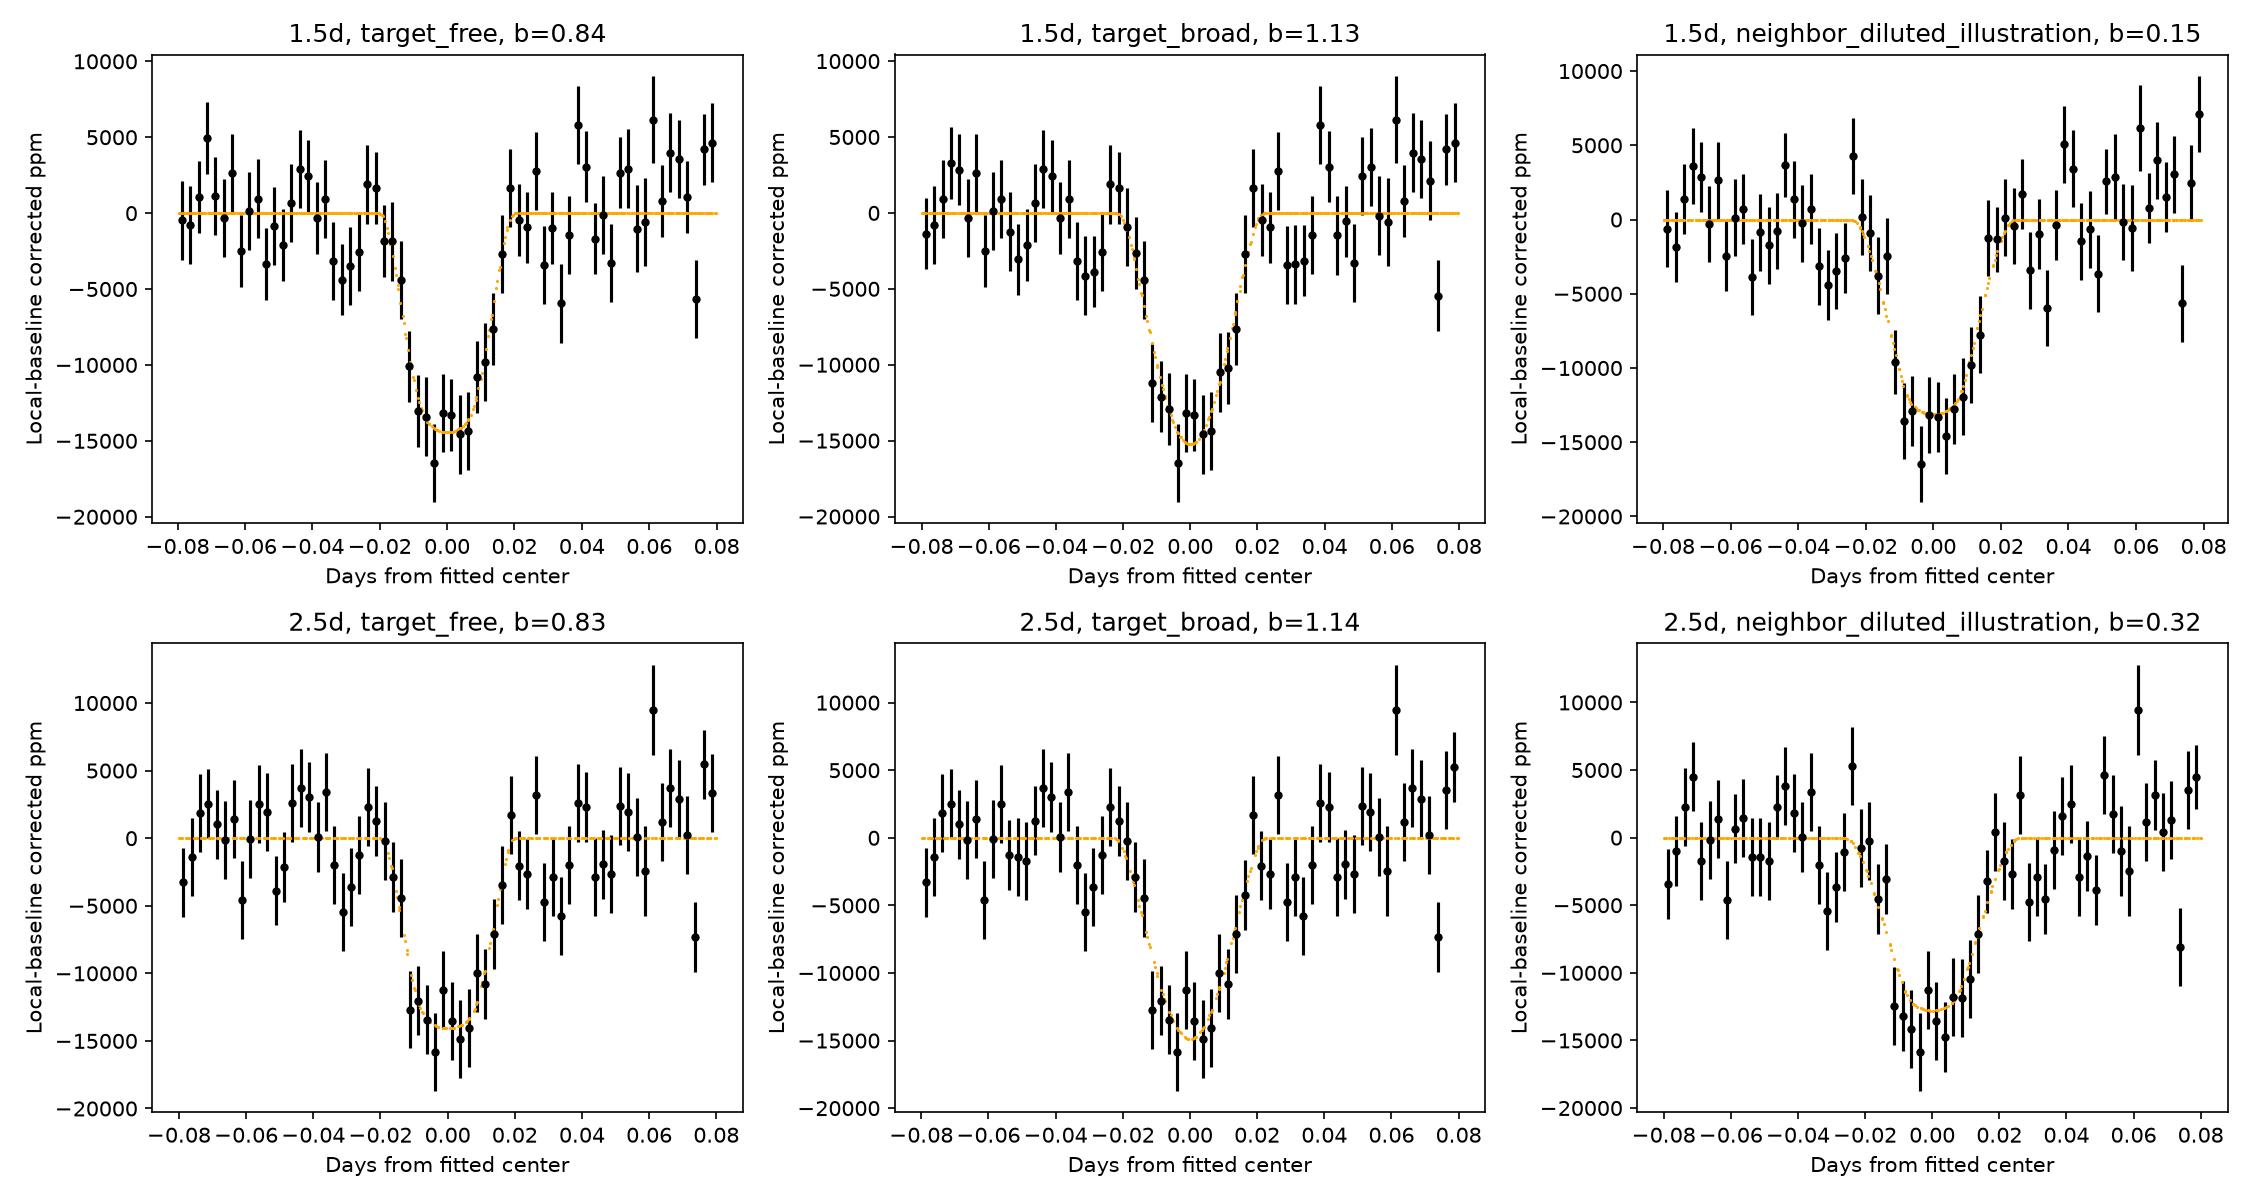
\includegraphics[width=\linewidth]{figures/241-physical.png}
\caption{Conditional physical fits to the same sector-92 observations of
TIC 241928959. Rows use the 1.5- and 2.5-day detrending windows; columns show
a target model with free orbital scale, a target model with a broad scale
prior, and an illustrative diluted-neighbor model. Similar folded shapes
accommodate very different companion sizes and grazing geometries. The neighbor
model reaches its radius-ratio bound and does not span general stellar-eclipse
models. These fits supply no independently validated planet radius.}
\label{fig:241physical}
\end{figure}

\subsection{TIC 469309982: mixed recurrence and a seasonal secondary concern}
\label{sec:tic469}
% Evidence: results/followup-469309982-20261011/ASSESSMENT.md
% results/season-out-469309982-20261011/ASSESSMENT.md

The four-sector weak-seed refinement uses sectors 9, 10, 36 and 37 and selects
$P=2.890464274$~d, a 0.144-day duration and a fitted depth of 138~ppm. Sector 64
at the unchanged nominal clock gives $75.8\pm26.2$~ppm. Its propagated timing
spread, 0.12347~d, exceeds the allowed half-duration of 0.072~d. A previously
saved alternative gives $133.4\pm26.2$~ppm, but this maximum across nine
correlated clocks cannot replace the nominal prediction. Sector 63, evaluated
using the clock selected after examining sector 64, is also weak:
$82\pm28$~ppm, falling to 21~ppm when one event is omitted.

Only one of six retrospective season-out comparisons passes both the original
recovery and timing conditions: the 1.5-day detrending predicts the omitted
sectors 36/37 at $129.7\pm22.6$~ppm with a 0.0525-day timing spread
(Figure~\ref{fig:469seasons}). The corresponding 2.5-day result is positive,
$136.7\pm23.5$~ppm, but separated accepted aliases expand its spread to
1.5706~d. All observations were previously inspected, the folds overlap, and
the discovery seed uses sectors 9/10 even when that season is omitted.

% Evidence: results/secondary-seasons-469309982-20261011/ASSESSMENT.md
% results/prf-motion-469309982-20261011/ASSESSMENT.md
A possible half-phase secondary is concentrated in sectors 36/37:
$87.8\pm22.7$~ppm at the 1.5-day window, compared with $24.0\pm22.6$ and
$-0.5\pm19.7$~ppm in the earlier and later seasons. This remains a concern
rather than a repeatable binary eclipse. Image models often favor neighbor
TIC 469309967, but substantial residuals and failures on known-planet controls
prevent a reliable source assignment.

% Evidence: results/new-epochs-469309982-96166003-20261012/ASSESSMENT.md
Sector 90 gives $-54.3\pm31.6$~ppm at the primary refined clock and
$14.1\pm33.8$~ppm at the alternate refined clock. Positive measurements at
the original unprofiled seed are retained without substitution
(Figure~\ref{fig:469961new}). Timing is inadequate and expected formal
sensitivity is below $5\sigma$, so this does not establish either recovery or
exclusion. The exact-source open-cluster reference supplies no useful age
prior.\footnote{TIC 469309982 is HD 300413. Its row in the checked Platais 8
membership table reports membership probability 0.00; bibliographic inclusion
is not cluster membership.}

\begin{figure}[p]
\centering
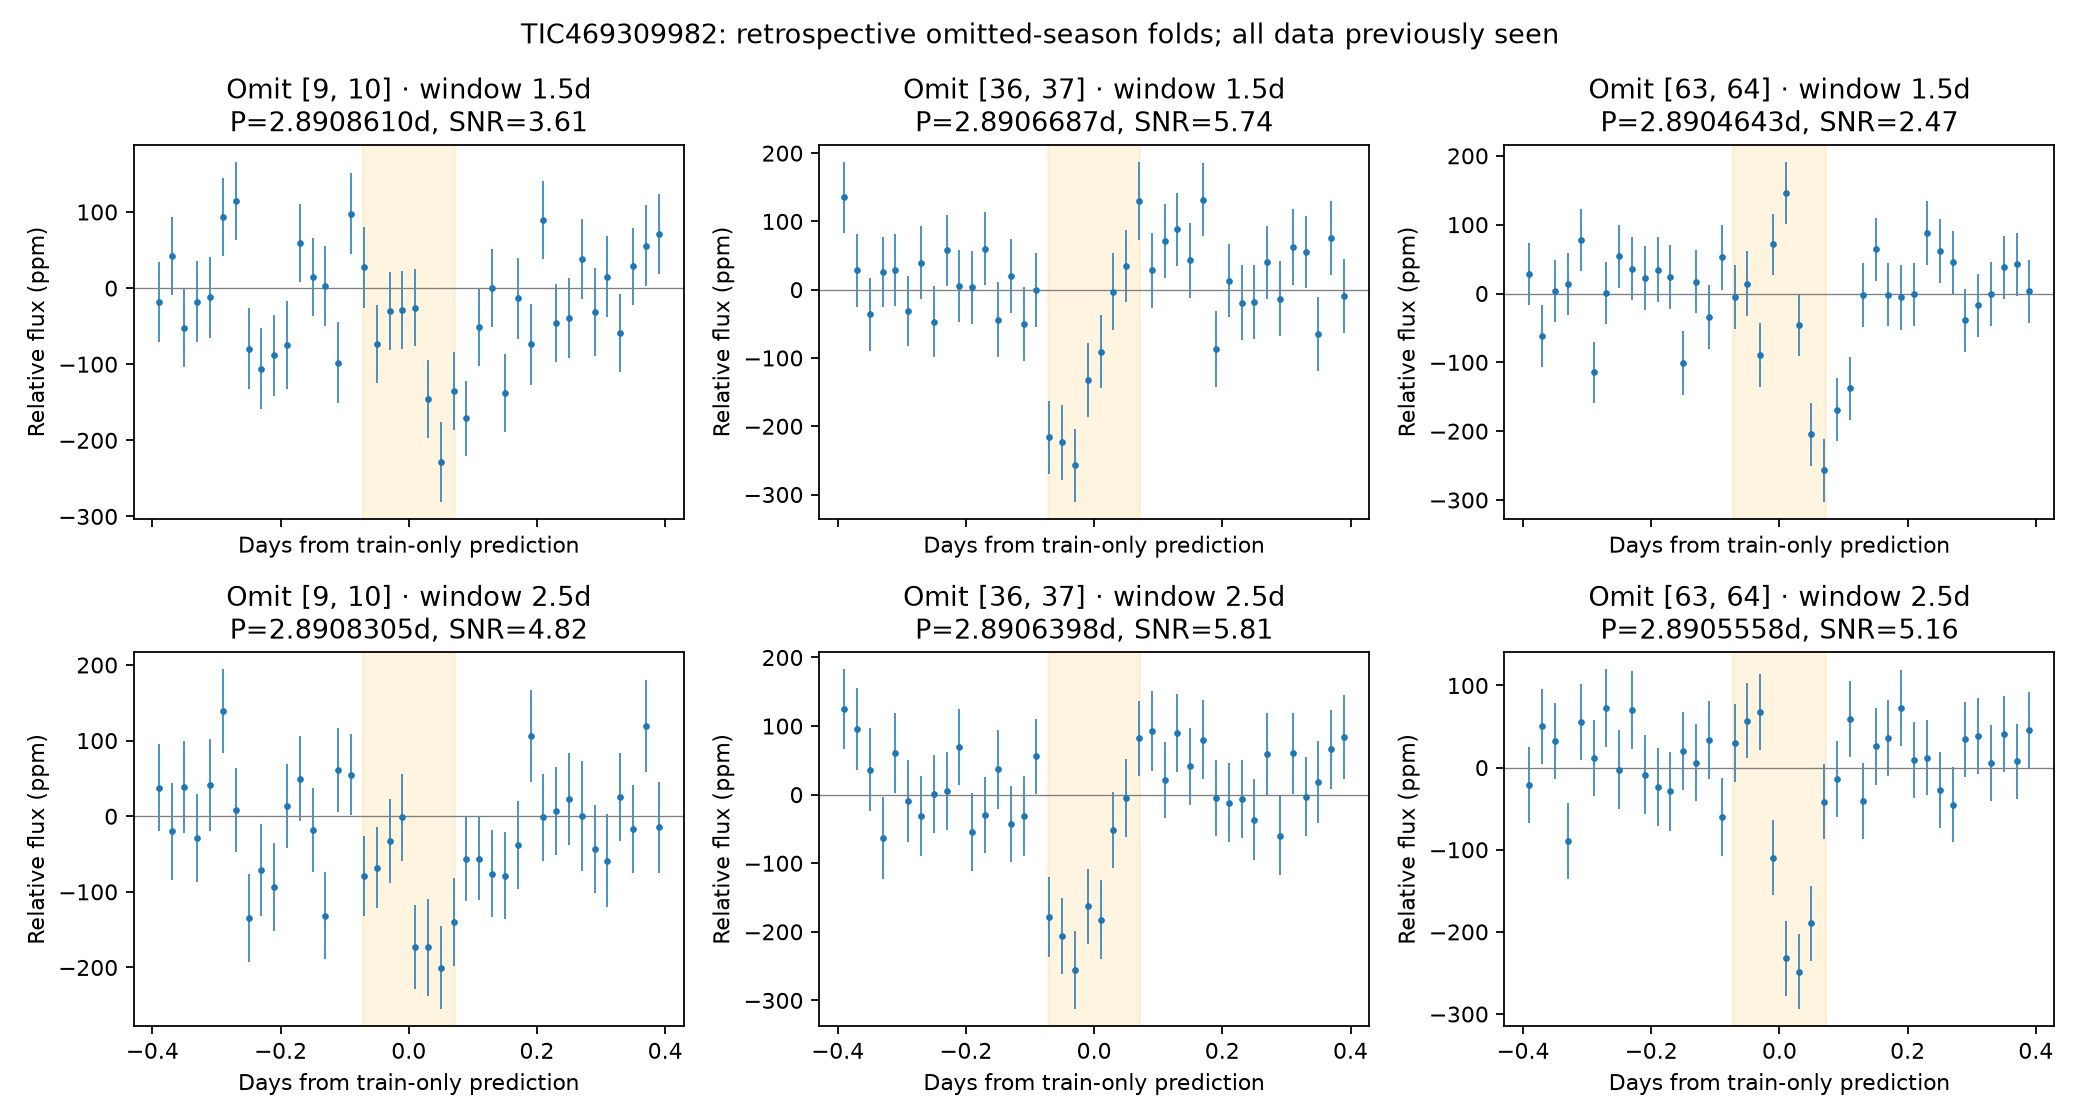
\includegraphics[width=\linewidth]{figures/469-seasons.png}
\caption{Retrospective omitted-season measurements for TIC 469309982.
Columns omit sectors 9/10, 36/37 and 63/64; rows use two detrending windows.
The shaded regions show the predicted boxes. Only the upper middle comparison
passes both timing and recovery gates. The other five remain timing-inconclusive,
including nominally strong lower-row features. All data were already inspected;
the seed and overlapping training sets prevent interpreting these as independent
blind discoveries. Displayed formal signal-to-noise values omit correlated
noise and clock uncertainty.}
\label{fig:469seasons}
\end{figure}

\subsection{TIC 96166003: positive depths depend on the clock}
\label{sec:tic961}
% Evidence: results/review-96166003-20261011/ASSESSMENT.md
% results/expanded-96166003-20261012/ASSESSMENT.md
% results/heldout-96166003-s59-20261012/ASSESSMENT.md

The original sectors 43/44 contain a compact approximately 0.955-day signal,
with fixed-clock local depths near 280~ppm under both detrendings. Sector 19
provides only weak, timing-inconclusive measurements. Once it becomes training,
the expanded primary clock is $P=0.955530474$~d with duration 0.05952~d;
the alternative selects $P=0.955279111$~d and duration 0.048~d. All accepted
profile islands remain preserved.

In sector 59 the primary predicts $264.9\pm51.9$~ppm, whereas the expanded
alternative gives $-72.4\pm62.4$~ppm and the two original-discovery comparisons
also give negative depths. Every prediction fails its timing gate; the primary
spread is 1.34665~d. Crossing both fixed clocks with both detrendings and SAP/
PDCSAP products retains the primary dip and the alternative's near-zero or
negative result. Thus this disagreement follows the timing hypotheses more than
these processing choices, but does not identify the correct hypothesis.

% Evidence: results/new-epochs-469309982-96166003-20261012/ASSESSMENT.md
% results/prf-96166003-20261012/ASSESSMENT.md
New sector 86 gives $248.2\pm100.7$~ppm at the expanded primary and
$7.2\pm134.0$~ppm at its alternative. All six retained comparisons are
low-sensitivity and timing-inconclusive (Figure~\ref{fig:961new}). Discovery
images favor the target nominally, but including faint neighbors changes some
sector-43 rankings. A physically viable diluted-binary alternative remains.
Neither the photometry nor template preferences securely establish a host.
A bibliographic planet-table association is also uninformative.\footnote{The
exact TIC 96166003 row in the checked TESS yield paper describes a simulated
15.592607-day planet, not an observed planet. It neither validates nor
invalidates the approximately 0.955-day signal investigated here.}

% Evidence: results/reliability-469309982-20261012/ASSESSMENT.md
% results/reliability-96166003-20261012/ASSESSMENT.md
For each of these two shallow signals, bounded block controls give zero
exceedances in 40 draws separately for each of three block models. Each
conditional 95\% Monte Carlo interval extends to 8.81\%; counts are not pooled.
These tests condition on selected targets and timing families and cannot supply
survey false-alarm probabilities or planet odds.

\begin{figure}[p]
\centering
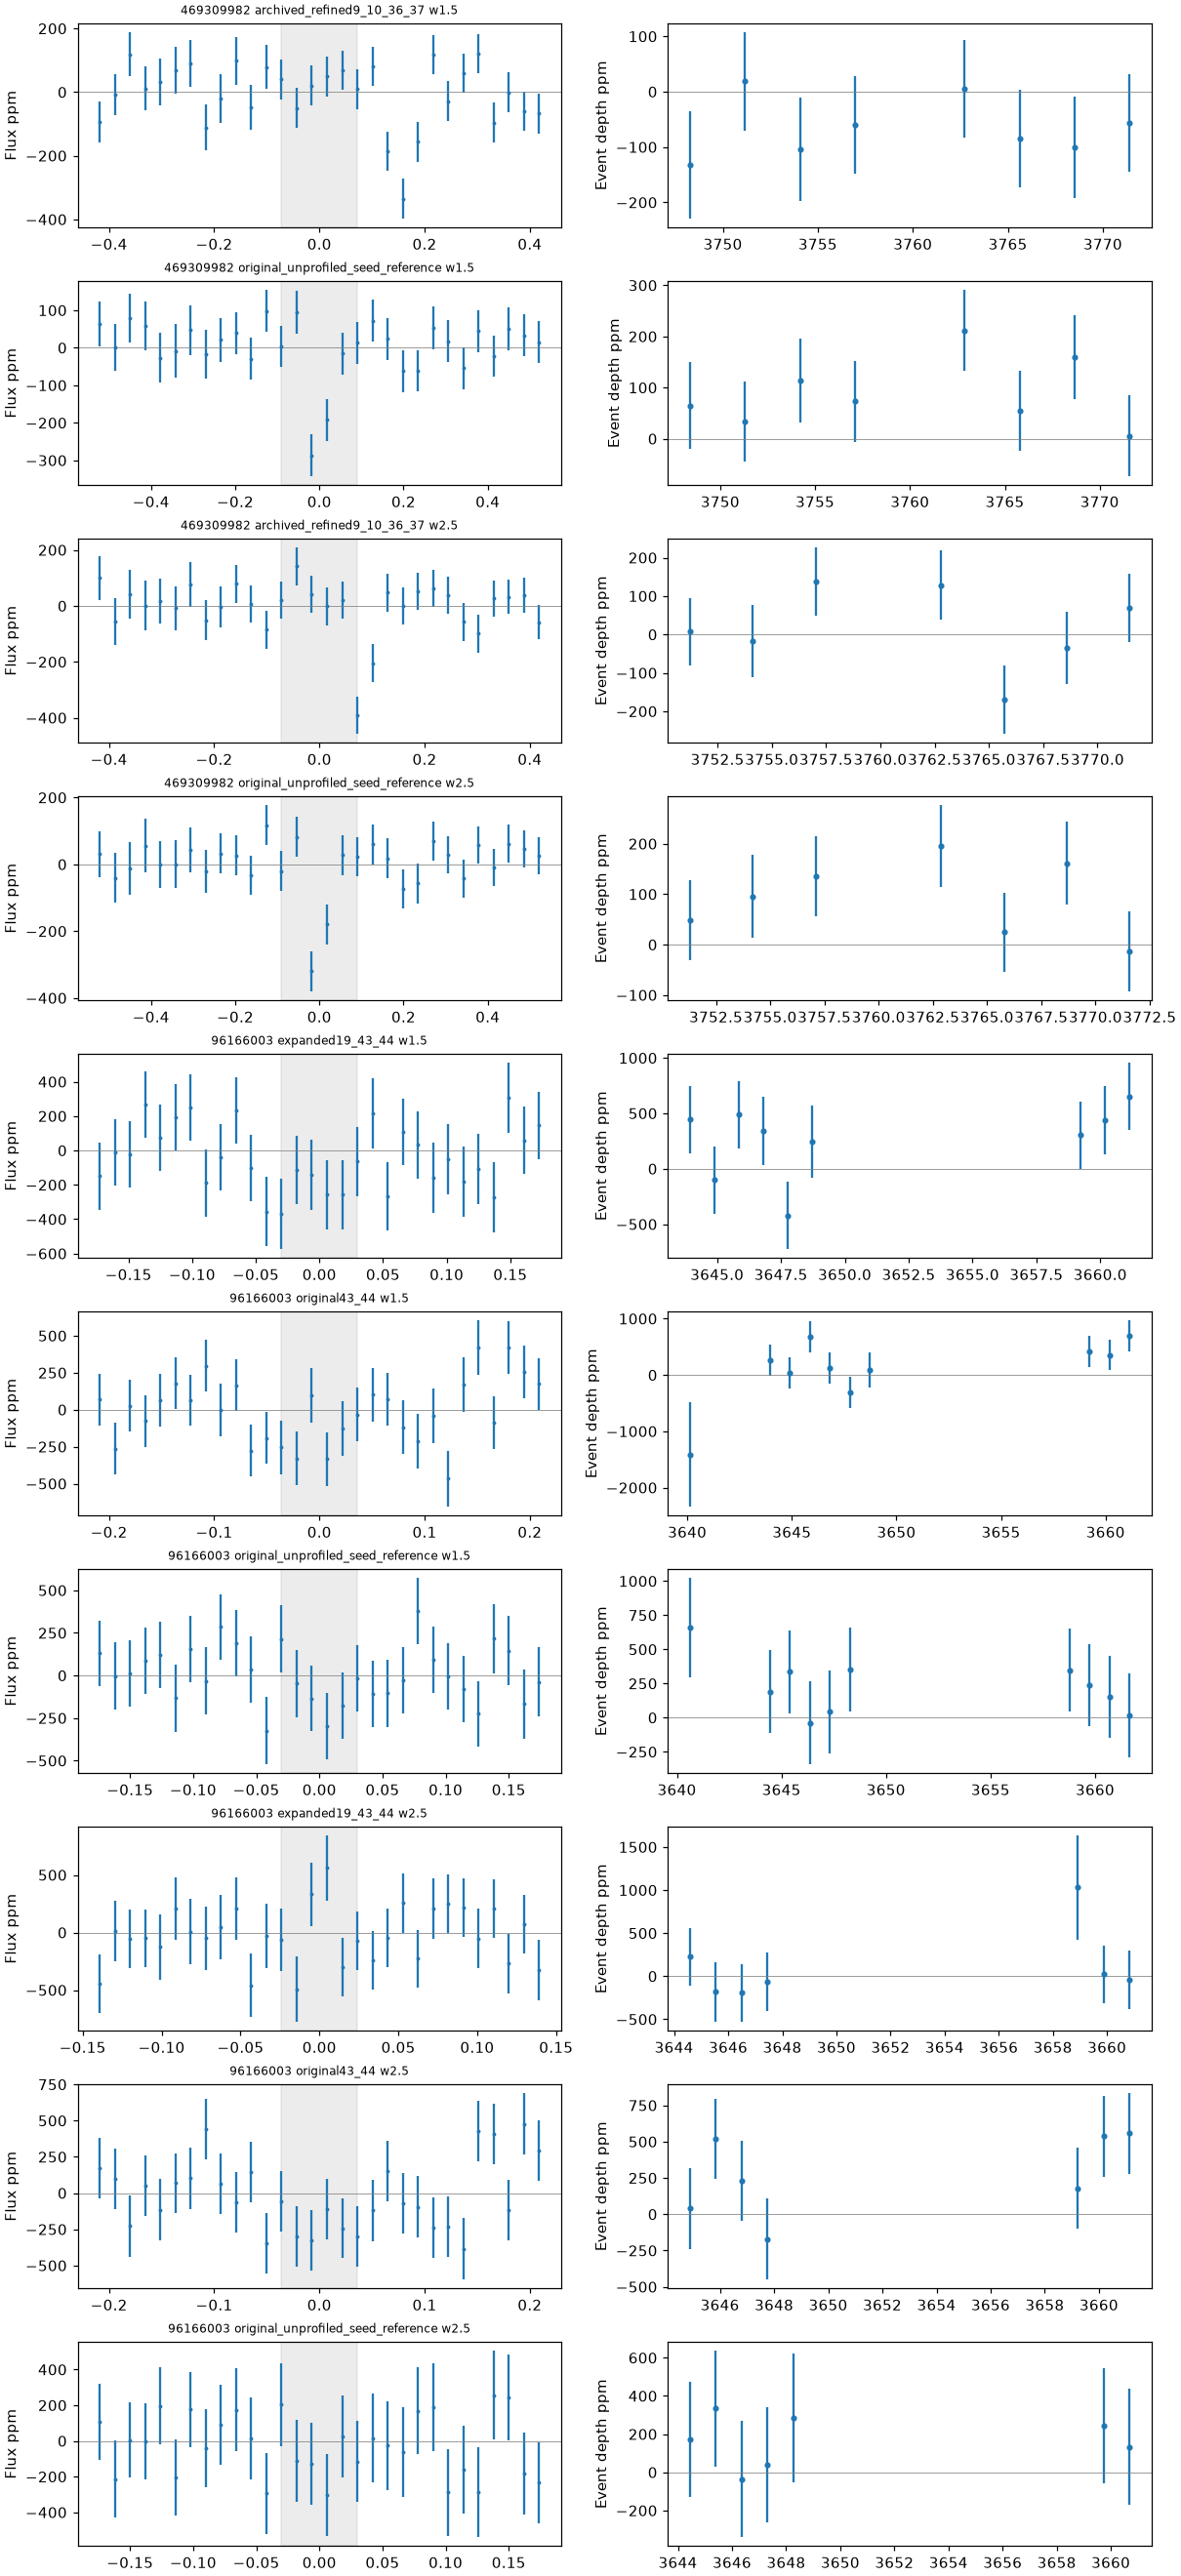
\includegraphics[width=\linewidth,trim=0 1036.8bp 0 0,clip]{figures/469-961-new.png}
\caption{The four saved clock comparisons for TIC 469309982 sector 90.
Left panels show fixed-clock folds (days from the predicted midpoint); right
panels show individual-event depths at centers in BTJD.
Positive depth denotes dimming. The primary result is negative. Profiled
clocks fail timing precision, unprofiled seed references are ineligible for
recovery, and expected formal sensitivity is below $5\sigma$ in every row.
This reproduces the upper four rows of the original ten-row chart; the lower
six rows are shown separately in Figure~\ref{fig:961new} for readability.}
\label{fig:469961new}
\end{figure}

\begin{figure}[p]
\centering
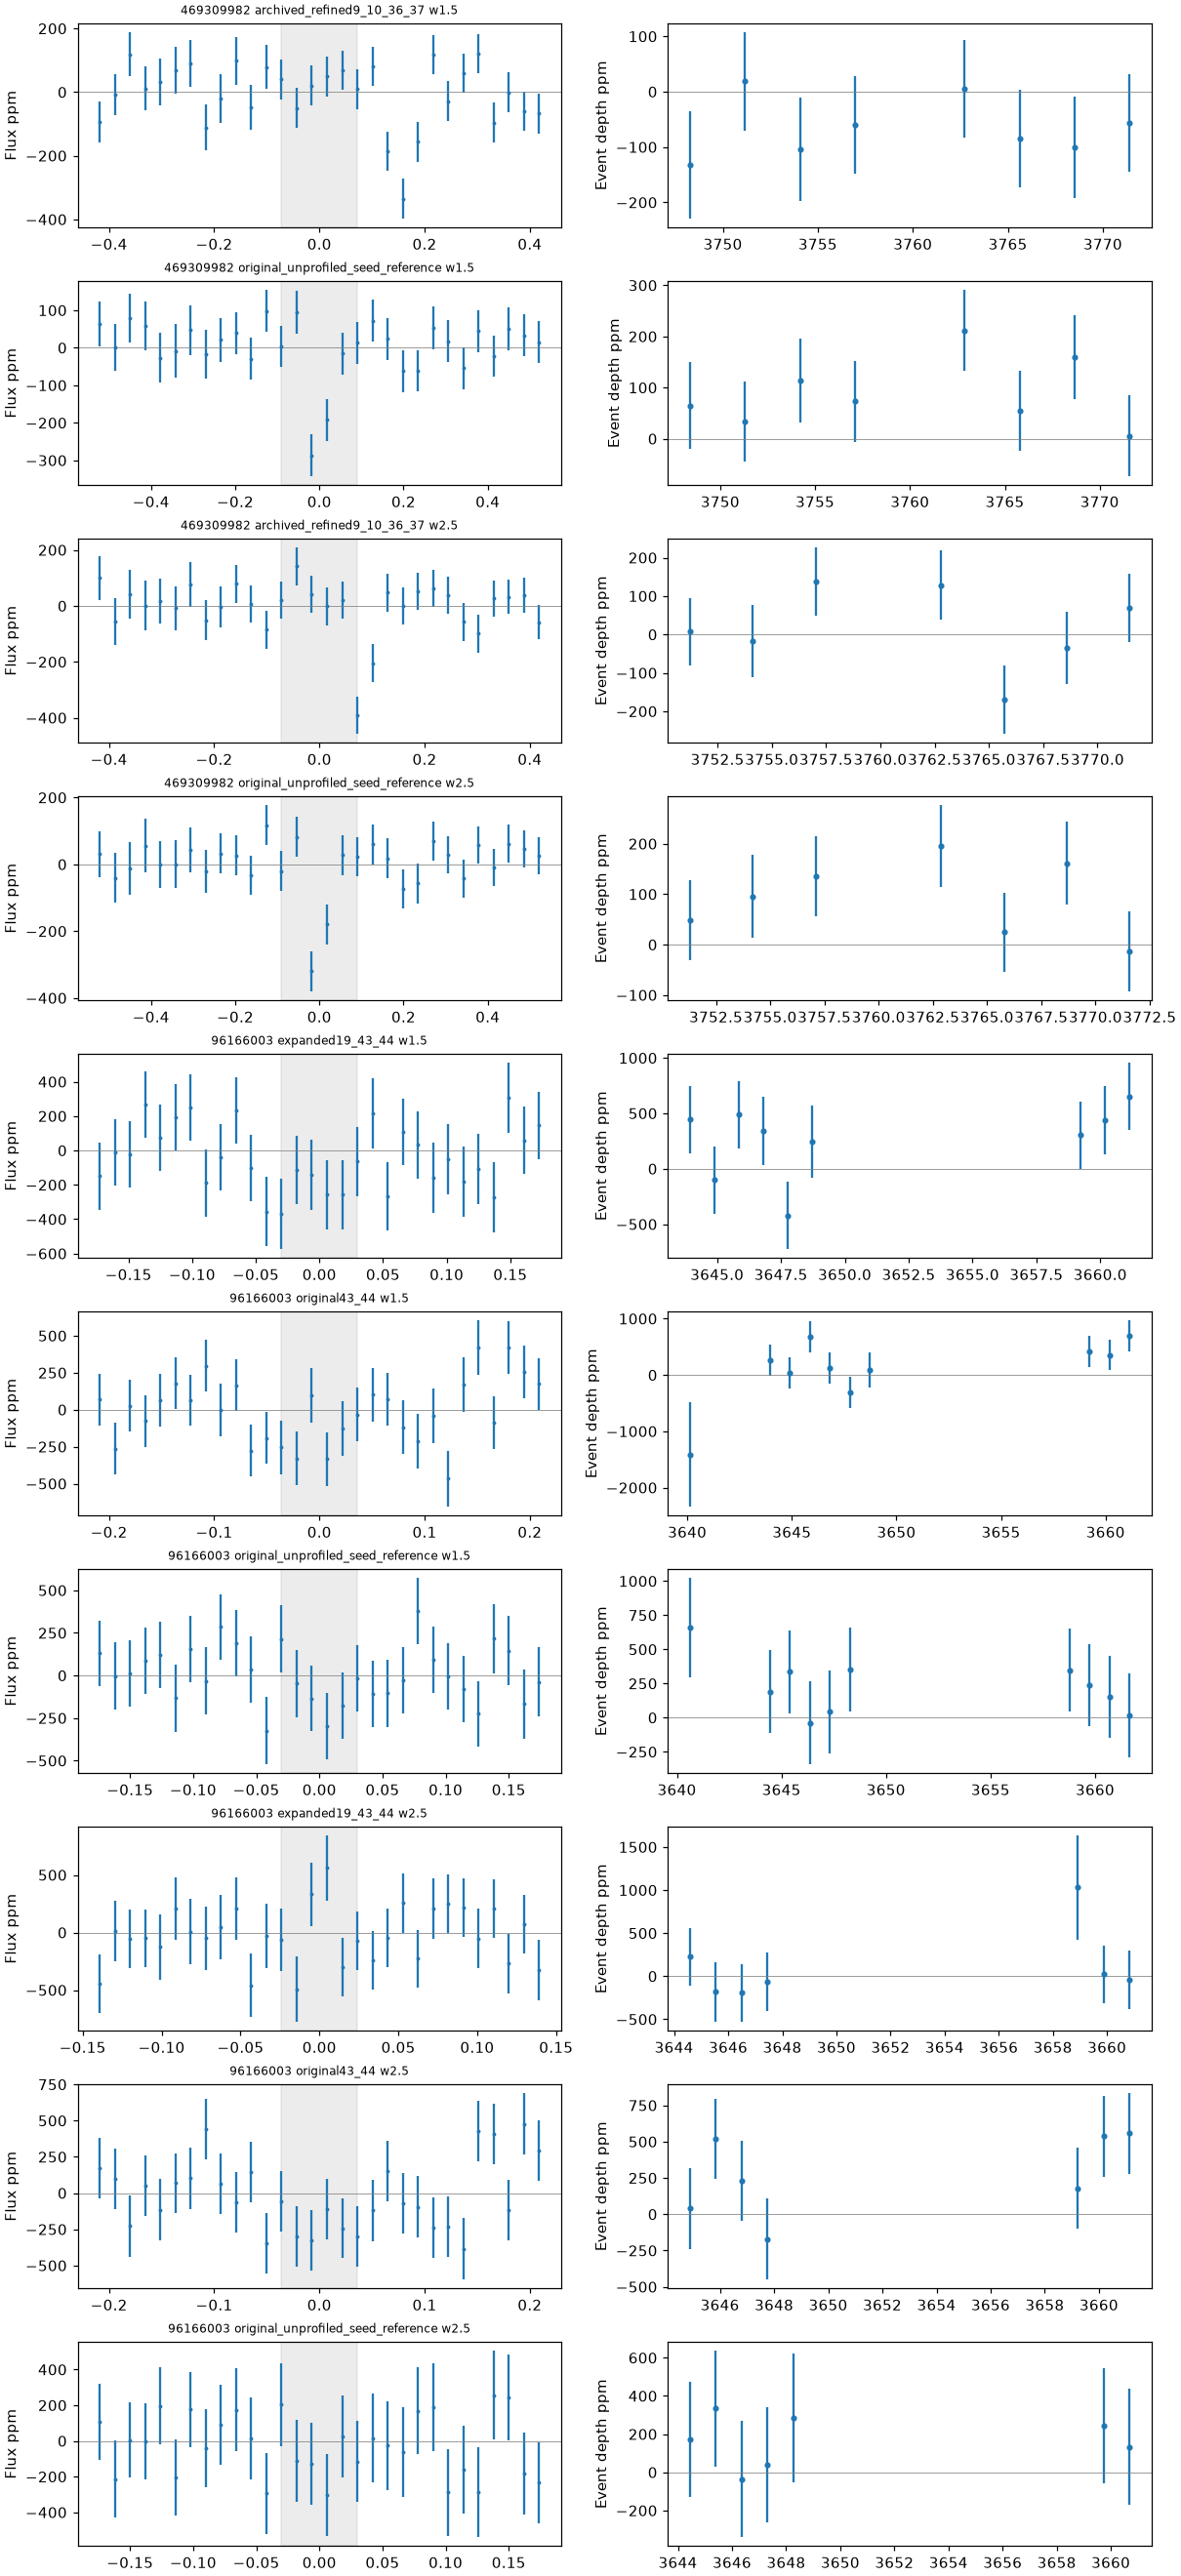
\includegraphics[width=\linewidth,height=0.78\textheight,keepaspectratio,trim=0 0 0 691.2bp,clip]{figures/469-961-new.png}
\caption{The six saved clock comparisons for TIC 96166003 sector 86,
reproducing the lower six rows of the same original chart as
Figure~\ref{fig:469961new}. The primary is weak, and the expanded alternative
is near zero. Left abscissae are days from the predicted midpoint; right
abscissae are event centers in BTJD. Profiled clocks fail timing precision, unprofiled seed references
are ineligible for recovery, and expected formal sensitivity is below
$5\sigma$ in every row. Repeated reductions share photons; none passes the
original recovery requirements. Only page layout has changed.}
\label{fig:961new}
\end{figure}

\subsection{TIC 5546257: resolved-neighbor variability strengthens contamination}
\label{sec:tic554}
% Evidence: results/followup-5546257-20261011/ASSESSMENT.md
% results/new-epochs-5546257-20261012/ASSESSMENT.md

The expanded pre-sector-62 clock, $P=1.767290230$~d and duration 0.133056~d,
gives $386.2\pm30.1$~ppm in sector 62. The timing spread, 0.07203~d, narrowly
exceeds the allowed 0.06653~d. Newly opened QLP sectors 89 and 99 retain nominal
clock dips of $271\pm28$ and $239\pm33$~ppm, but their timing spreads also
fail the original gate. The coarse discovery seed gives negative depths.
Different extraction methods and apertures prevent interpreting these depth
changes as intrinsic evolution or improved source attribution.

% Evidence: results/prf-motion-5546257-s62-20261011/ASSESSMENT.md
% results/contaminant-clock-5546257-20261012/ASSESSMENT.md
Sector-62 source-plus-motion models favor neighboring TIC 5546242:
$\chi^2=259.24/126$, compared with $776.24/126$ for the target. All 13 event
omissions and 10 of 13 individual images favor the neighbor, whose exact Gaia
source is classified as an eclipsing binary. However, its catalog period,
7.248263937 TCB days, and the tested simple harmonics do not explain the
selected TESS train. The closest period division, $P/4=1.812065956$~d, is
2.53\% longer. This mismatch prevents claiming a complete catalog-clock
explanation, while leaving contamination plausible.

% Evidence: results/extension-402358350-5546257-20261012/ASSESSMENT.md
Resolved Gaia epoch photometry of that neighbor supplies stronger adverse
evidence (Figure~\ref{fig:554gaia}). All five nominal in-window measurements
at the unchanged refined TESS clock dim, with relative depth
$16.343\pm0.192\%$; a sixth dim point lies just outside. The backward timing
spread remains too large, and the 13 saved timing alternatives include only
two to six of the conspicuous dim points. The published Gaia model explains
most samples but leaves one notable discrepancy. Sparse sampling permits a
possible catalog alias; no period was refitted to select that explanation.
The neighbor association is strengthened, although its exact orbit, aperture
dilution and quantitative explanation of the TESS signal remain unresolved.

\begin{figure}[p]
\centering
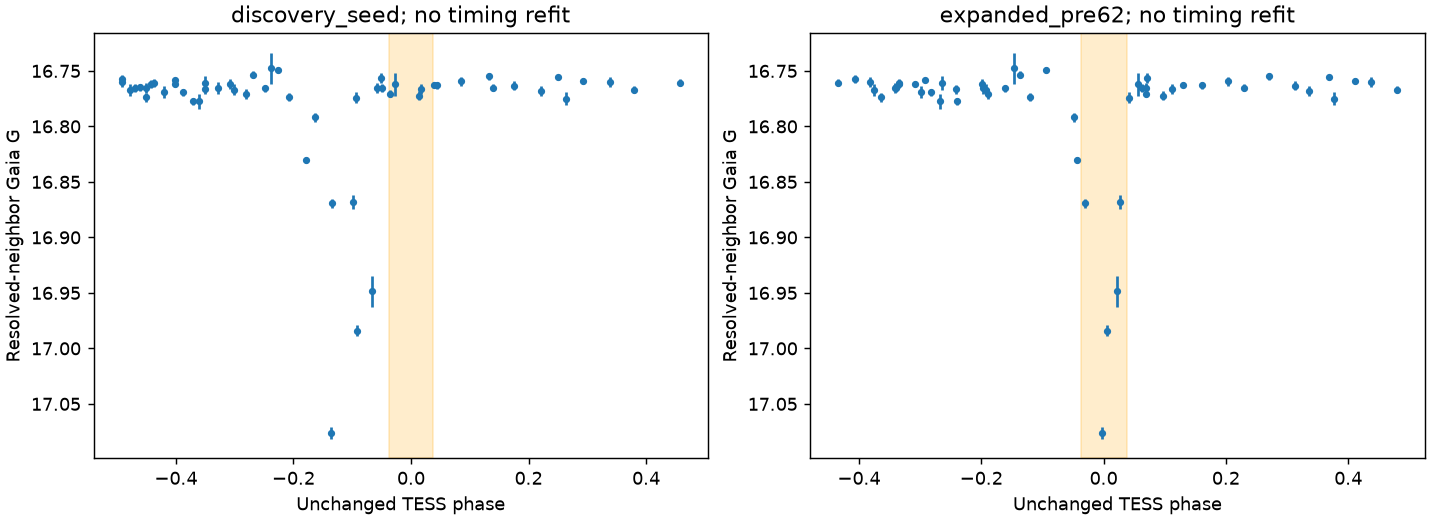
\includegraphics[width=\linewidth]{figures/554-gaia.png}
\caption{Resolved Gaia $G$ measurements of TIC 5546242, the binary neighbor
favored by TIC 5546257 difference images. Left: unchanged coarse discovery
clock. Right: unchanged expanded pre-sector-62 clock. The latter aligns five
dim points within the frozen window and a sixth nearby, supporting
contamination. The backward timing gate still fails, and alternate saved
profiles do not all align the same points. Neither this nominal alignment nor
the catalog model settles the period alias or the TESS dilution. These are
neighbor measurements, not independently confirmed target transits.}
\label{fig:554gaia}
\end{figure}

\clearpage

\section{Interpretation and follow-up}\label{sec:discussion}
The evidence supports different levels of recurrence, without completing the chain from a selected dip to a planetary discovery. TIC~80387959 has the clearest prospective recurrence: its fixed earlier clock recovered dimming in two later sectors, and retrospective native-cadence fits preserve the dip across six sectors. TIC~402358350 has the strongest local-baseline stress test, but its later-sector timing gate fails. The other fields preserve useful patterns or contamination evidence with weaker independent recurrence. These distinctions should guide follow-up rather than be collapsed into a numerical ranking of planet probabilities.

Several checks constrain only particular alternatives. A missing exact-half-phase secondary does not exclude an eccentric or diluted stellar binary. A sinusoidal nuisance model does not span general stellar variability. A normal single spectrum or two consistent survey velocities does not exclude an eclipsing companion. Sparse photometry outside the relevant timing envelope cannot veto an eclipse. Catalog non-matches and failed archive queries must remain separate: neither proves that a star is constant, single, or previously unstudied. Qualitative follow-up priority and agreement among computational checks are not independent validation.

Resolved, time-resolved photometry is the most direct next experiment for the two priority fields. It should measure the target and all viable neighbors through the entire predicted event with sufficient out-of-event baseline. A target-centered dimming would still require constraints on unresolved companions. Appropriate spectroscopy and high-resolution imaging could then reduce blend and stellar-companion ambiguity, as in established validation workflows \citep{giacalone2022,cacciapuoti2022,eisner2021}. Candidate-specific error and throughput calibration are necessary before interpreting an image-model preference as a source probability.

The retained planning packet contains 47 nominal TIC~80387959 windows and 17 nominal TIC~402358350 windows through April~2027. These are predictions, not observed events or telescope allocations. Selected-profile timing envelopes plus one hour of baseline on each side require approximately 5.6 hours for TIC~80387959 and 17.5--18.5 hours for TIC~402358350. They are heuristic timing ranges, not calibrated confidence bounds, and older alternative clocks can imply larger uncertainty. No full conservative LCO one-meter track passes the retained mount-margin assessment. One T17 date passes the tested sky geometry, but the actual instrument horizon, mount constraints, access, and precision remain unverified. No observing time is secured and no inquiry has been sent. A short non-detection under these conditions would be inconclusive.

\section{Conclusions}
We retain six unresolved TESS signal assessments and an explicit record of the tests that favor or weaken their interpretations. The fixed-clock later-sector recovery of TIC~80387959 and the eight-event baseline robustness of TIC~402358350 justify additional investigation. Their host stars and physical causes remain uncertain. TIC~241928959 lacks a second epoch and permits substantially different companion interpretations; TIC~469309982 and TIC~96166003 have weak or clock-dependent recurrence; TIC~5546257 has strengthened evidence for a neighboring eclipsing source without a complete alias and dilution explanation. None is validated or confirmed as a planet, and novelty is unestablished. The value of the present release is a reproducible starting point for decisive follow-up, including the negative evidence needed to design it.

\section*{Data, code, and provenance}
The code, saved measurements, figures, run plans, input manifests, and verification reports are available at \url{https://github.com/relh/exoplanet}. This manuscript uses the scientific state assessed on 13 October 2026; its preparation did not open new observing epochs or run a new candidate search. The public evidence baseline is commit \texttt{0537d585d}. Appendix~\ref{app:evidence} links the principal reports. The accompanying \texttt{evidence-manifest.json} records full file paths and SHA-256 hashes for every reproduced figure and the selected numerical, plan, source, and assessment records. The standalone source package includes the figures needed to compile this paper; the full repository retains the larger evidence archive and third-party data credits.

The publication cleanup removed operational host/session metadata and authentication parameters from expired signed download URLs. Original frozen-file hashes are retained, with original-to-sanitized mappings in \path{docs/privacy-edits.json} and \path{docs/release-history-redactions.json}. Edited plans are not new pre-access freezes. Exact original-byte verification can require the translation or the retained private originals; numerical experiment fields and scientific conclusions were preserved. Raw downloads remain outside Git and are identified by the run manifests. Reproducing arithmetic from a saved dataset does not independently validate its scientific model.

\section*{Acknowledgments and software}
This work uses public TESS observations, TESS-SPOC and QLP products from MAST, ESA Gaia data processed by the Gaia Data Processing and Analysis Consortium, and the external surveys credited in the individual reports, including RAVE, SkyMapper, and ZTF. TESS mission funding is provided by NASA's Science Mission Directorate. The TESS-SPOC dataset is identified by \href{https://doi.org/10.17909/t9-wpz1-8s54}{doi:10.17909/t9-wpz1-8s54}; product-level identities and retrieval hashes remain in the research archive. Third-party material retains its original terms and attribution. Software includes Python, NumPy, SciPy, Matplotlib, Astropy \citep{astropy2022}, batman \citep{kreidberg2015}, and TRICERATOPS \citep{giacalone2021}. AI-assisted tools were used in preparing this manuscript; their output and agreement are not independent scientific validation. The author is responsible for the reported interpretations.

\clearpage
\bibliographystyle{plainnat}
\bibliography{references}
\clearpage
\appendix
\section{Evidence inventory}\label{app:evidence}
The following reports provide the complete measurements, alternatives, quality failures, and run-specific verification. Links are pinned to the public evidence baseline. File hashes and figure-to-source mappings are in the accompanying manifest; the reports link the underlying plans, numerical arrays, and source snapshots. Historical conclusions are superseded only where the current assessment says so.
\footnotesize
\begin{longtable}{@{}>{\raggedright\arraybackslash}p{0.055\textwidth}>{\raggedright\arraybackslash}p{0.23\textwidth}>{\raggedright\arraybackslash}p{0.66\textwidth}@{}}
\toprule ID & Evidence & Repository path \\
\midrule\endhead
E01 & Scope and evidence index & \href{https://github.com/relh/exoplanet/blob/0537d585d10e428fad63b4b38f5b9822590b271a/CHECKED-RESULTS.md}{\nolinkurl{CHECKED-RESULTS.md}} \\
E02 & Search completion & \href{https://github.com/relh/exoplanet/blob/0537d585d10e428fad63b4b38f5b9822590b271a/results/scoped-completion-20261012/ASSESSMENT.md}{\nolinkurl{results/scoped-completion-20261012/ASSESSMENT.md}} \\
E03 & Solar selection & \href{https://github.com/relh/exoplanet/blob/0537d585d10e428fad63b4b38f5b9822590b271a/results/solar-radius-pilot-selection-20261011/ASSESSMENT.md}{\nolinkurl{results/solar-radius-pilot-selection-20261011/ASSESSMENT.md}} \\
E04 & Solar ledger & \href{https://github.com/relh/exoplanet/blob/0537d585d10e428fad63b4b38f5b9822590b271a/results/solar-radius-lead-audit-20261011/ASSESSMENT.md}{\nolinkurl{results/solar-radius-lead-audit-20261011/ASSESSMENT.md}} \\
E05 & Weak-seed review & \href{https://github.com/relh/exoplanet/blob/0537d585d10e428fad63b4b38f5b9822590b271a/results/weak-seed-audit-20261011/ASSESSMENT.md}{\nolinkurl{results/weak-seed-audit-20261011/ASSESSMENT.md}} \\
E06 & Faint QLP expansion & \href{https://github.com/relh/exoplanet/blob/0537d585d10e428fad63b4b38f5b9822590b271a/results/qlp-faint-expanded-20261010/ASSESSMENT.md}{\nolinkurl{results/qlp-faint-expanded-20261010/ASSESSMENT.md}} \\
E07 & Reserved-data exception & \href{https://github.com/relh/exoplanet/blob/0537d585d10e428fad63b4b38f5b9822590b271a/results/solar-radius-ranks3920-4432-20261011/ASSESSMENT.md}{\nolinkurl{results/solar-radius-ranks3920-4432-20261011/ASSESSMENT.md}} \\
E08 & Known-host controls & \href{https://github.com/relh/exoplanet/blob/0537d585d10e428fad63b4b38f5b9822590b271a/results/solar-radius-positive-controls-20261011/ASSESSMENT.md}{\nolinkurl{results/solar-radius-positive-controls-20261011/ASSESSMENT.md}} \\
E09 & Shallow injections & \href{https://github.com/relh/exoplanet/blob/0537d585d10e428fad63b4b38f5b9822590b271a/results/solar-radius-shallow-injections-20261011/ASSESSMENT.md}{\nolinkurl{results/solar-radius-shallow-injections-20261011/ASSESSMENT.md}} \\
E10 & 803 frozen prediction & \href{https://github.com/relh/exoplanet/blob/0537d585d10e428fad63b4b38f5b9822590b271a/results/followup-80387959-qlp90-100-20261009/heldout.json}{\nolinkurl{results/followup-80387959-qlp90-100-20261009/heldout.json}} \\
E11 & 803 native profiles & \href{https://github.com/relh/exoplanet/blob/0537d585d10e428fad63b4b38f5b9822590b271a/results/strongest-80387959-shape-20261012/ASSESSMENT.md}{\nolinkurl{results/strongest-80387959-shape-20261012/ASSESSMENT.md}} \\
E12 & 402 frozen sector 81 & \href{https://github.com/relh/exoplanet/blob/0537d585d10e428fad63b4b38f5b9822590b271a/results/heldout-402358350-s81-20261011/ASSESSMENT.md}{\nolinkurl{results/heldout-402358350-s81-20261011/ASSESSMENT.md}} \\
E13 & 402 local baselines & \href{https://github.com/relh/exoplanet/blob/0537d585d10e428fad63b4b38f5b9822590b271a/results/strongest-402358350-baselines-20261012/ASSESSMENT.md}{\nolinkurl{results/strongest-402358350-baselines-20261012/ASSESSMENT.md}} \\
E14 & 803 noise audit & \href{https://github.com/relh/exoplanet/blob/0537d585d10e428fad63b4b38f5b9822590b271a/results/paper-vetting-80387959-20261012/ASSESSMENT.md}{\nolinkurl{results/paper-vetting-80387959-20261012/ASSESSMENT.md}} \\
E15 & 402 noise audit & \href{https://github.com/relh/exoplanet/blob/0537d585d10e428fad63b4b38f5b9822590b271a/results/paper-vetting-402358350-20261012/ASSESSMENT.md}{\nolinkurl{results/paper-vetting-402358350-20261012/ASSESSMENT.md}} \\
E16 & Neighbor light budgets & \href{https://github.com/relh/exoplanet/blob/0537d585d10e428fad63b4b38f5b9822590b271a/results/paper-host-vetting-20261012/ASSESSMENT.md}{\nolinkurl{results/paper-host-vetting-20261012/ASSESSMENT.md}} \\
E17 & Image control failure & \href{https://github.com/relh/exoplanet/blob/0537d585d10e428fad63b4b38f5b9822590b271a/results/prf-137151335-20261011/ASSESSMENT.md}{\nolinkurl{results/prf-137151335-20261011/ASSESSMENT.md}} \\
E18 & Source instability & \href{https://github.com/relh/exoplanet/blob/0537d585d10e428fad63b4b38f5b9822590b271a/results/prf-80387959-event-stability-20261011/ASSESSMENT.md}{\nolinkurl{results/prf-80387959-event-stability-20261011/ASSESSMENT.md}} \\
E19 & Pointing controls & \href{https://github.com/relh/exoplanet/blob/0537d585d10e428fad63b4b38f5b9822590b271a/results/pointing-correction-controls-20261012/ASSESSMENT.md}{\nolinkurl{results/pointing-correction-controls-20261012/ASSESSMENT.md}} \\
E20 & Aperture controls & \href{https://github.com/relh/exoplanet/blob/0537d585d10e428fad63b4b38f5b9822590b271a/results/strongest-host-identifiability-20261012/ASSESSMENT.md}{\nolinkurl{results/strongest-host-identifiability-20261012/ASSESSMENT.md}} \\
E21 & TRICERATOPS results & \href{https://github.com/relh/exoplanet/blob/0537d585d10e428fad63b4b38f5b9822590b271a/results/triceratops-20261013/ASSESSMENT.md}{\nolinkurl{results/triceratops-20261013/ASSESSMENT.md}} \\
E22 & TRICERATOPS review & \href{https://github.com/relh/exoplanet/blob/0537d585d10e428fad63b4b38f5b9822590b271a/results/triceratops-review-20261013/ASSESSMENT.md}{\nolinkurl{results/triceratops-review-20261013/ASSESSMENT.md}} \\
E23 & Resolved SkyMapper & \href{https://github.com/relh/exoplanet/blob/0537d585d10e428fad63b4b38f5b9822590b271a/results/resolved-followup-803-20261013/ASSESSMENT.md}{\nolinkurl{results/resolved-followup-803-20261013/ASSESSMENT.md}} \\
E24 & Resolved ZTF & \href{https://github.com/relh/exoplanet/blob/0537d585d10e428fad63b4b38f5b9822590b271a/results/resolved-followup-402-20261013/ASSESSMENT.md}{\nolinkurl{results/resolved-followup-402-20261013/ASSESSMENT.md}} \\
E25 & 241 physical fits & \href{https://github.com/relh/exoplanet/blob/0537d585d10e428fad63b4b38f5b9822590b271a/results/physical-241928959-20261012/ASSESSMENT.md}{\nolinkurl{results/physical-241928959-20261012/ASSESSMENT.md}} \\
E26 & 469 season tests & \href{https://github.com/relh/exoplanet/blob/0537d585d10e428fad63b4b38f5b9822590b271a/results/season-out-469309982-20261011/ASSESSMENT.md}{\nolinkurl{results/season-out-469309982-20261011/ASSESSMENT.md}} \\
E27 & 469/961 new epochs & \href{https://github.com/relh/exoplanet/blob/0537d585d10e428fad63b4b38f5b9822590b271a/results/new-epochs-469309982-96166003-20261012/ASSESSMENT.md}{\nolinkurl{results/new-epochs-469309982-96166003-20261012/ASSESSMENT.md}} \\
E28 & 961 clock comparison & \href{https://github.com/relh/exoplanet/blob/0537d585d10e428fad63b4b38f5b9822590b271a/results/same-clock-96166003-20261012/ASSESSMENT.md}{\nolinkurl{results/same-clock-96166003-20261012/ASSESSMENT.md}} \\
E29 & 554 new epochs & \href{https://github.com/relh/exoplanet/blob/0537d585d10e428fad63b4b38f5b9822590b271a/results/new-epochs-5546257-20261012/ASSESSMENT.md}{\nolinkurl{results/new-epochs-5546257-20261012/ASSESSMENT.md}} \\
E30 & Pulsator and Gaia tests & \href{https://github.com/relh/exoplanet/blob/0537d585d10e428fad63b4b38f5b9822590b271a/results/extension-402358350-5546257-20261012/ASSESSMENT.md}{\nolinkurl{results/extension-402358350-5546257-20261012/ASSESSMENT.md}} \\
E31 & 554 catalog alias & \href{https://github.com/relh/exoplanet/blob/0537d585d10e428fad63b4b38f5b9822590b271a/results/contaminant-clock-5546257-20261012/ASSESSMENT.md}{\nolinkurl{results/contaminant-clock-5546257-20261012/ASSESSMENT.md}} \\
E32 & Six local baselines & \href{https://github.com/relh/exoplanet/blob/0537d585d10e428fad63b4b38f5b9822590b271a/results/event-baseline-six-20261012/ASSESSMENT.md}{\nolinkurl{results/event-baseline-six-20261012/ASSESSMENT.md}} \\
E33 & Companion metadata & \href{https://github.com/relh/exoplanet/blob/0537d585d10e428fad63b4b38f5b9822590b271a/results/companion-constraints-shortlist-20261012/ASSESSMENT.md}{\nolinkurl{results/companion-constraints-shortlist-20261012/ASSESSMENT.md}} \\
E34 & 803 spectroscopy & \href{https://github.com/relh/exoplanet/blob/0537d585d10e428fad63b4b38f5b9822590b271a/results/web-80387959-20261012/ASSESSMENT.md}{\nolinkurl{results/web-80387959-20261012/ASSESSMENT.md}} \\
E35 & Follow-up planning & \href{https://github.com/relh/exoplanet/blob/0537d585d10e428fad63b4b38f5b9822590b271a/results/followup-planning-20261013/ASSESSMENT.md}{\nolinkurl{results/followup-planning-20261013/ASSESSMENT.md}} \\
E36 & Observing access & \href{https://github.com/relh/exoplanet/blob/0537d585d10e428fad63b4b38f5b9822590b271a/results/observing-access-20261013/ASSESSMENT.md}{\nolinkurl{results/observing-access-20261013/ASSESSMENT.md}} \\
\bottomrule
\end{longtable}
\normalsize


\clearpage
\section{Additional diagnostic figures}\label{app:figures}
These figures retain noise, source-identification, external-photometry, and processing limitations alongside the primary light-curve evidence. Panels from the same exposures are dependent comparisons. Their error bars do not include all source, timing, or instrumental uncertainties.
\begin{figure}[htbp]
\centering
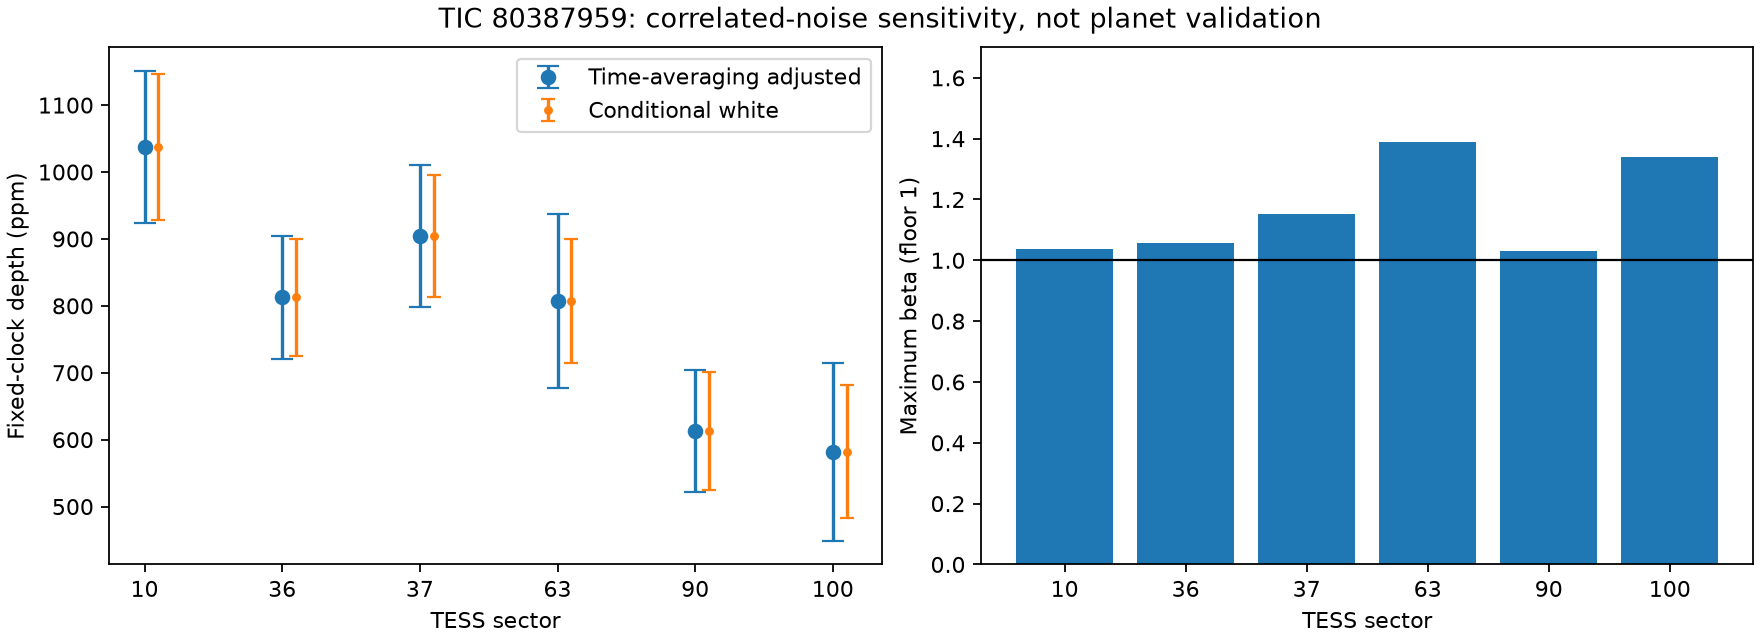
\includegraphics[width=\linewidth,height=0.72\textheight,keepaspectratio]{figures/803-noise.png}
\caption{TIC 80387959 time-averaging sensitivity. The six sector depths are retained while approximate error inflation and individual-event omissions reduce their apparent precision. The white-noise reference uses the same fitting design. Scalar inflation is not a complete correlated-noise model or a calibrated detection significance.}
\end{figure}
\begin{figure}[p]
\centering
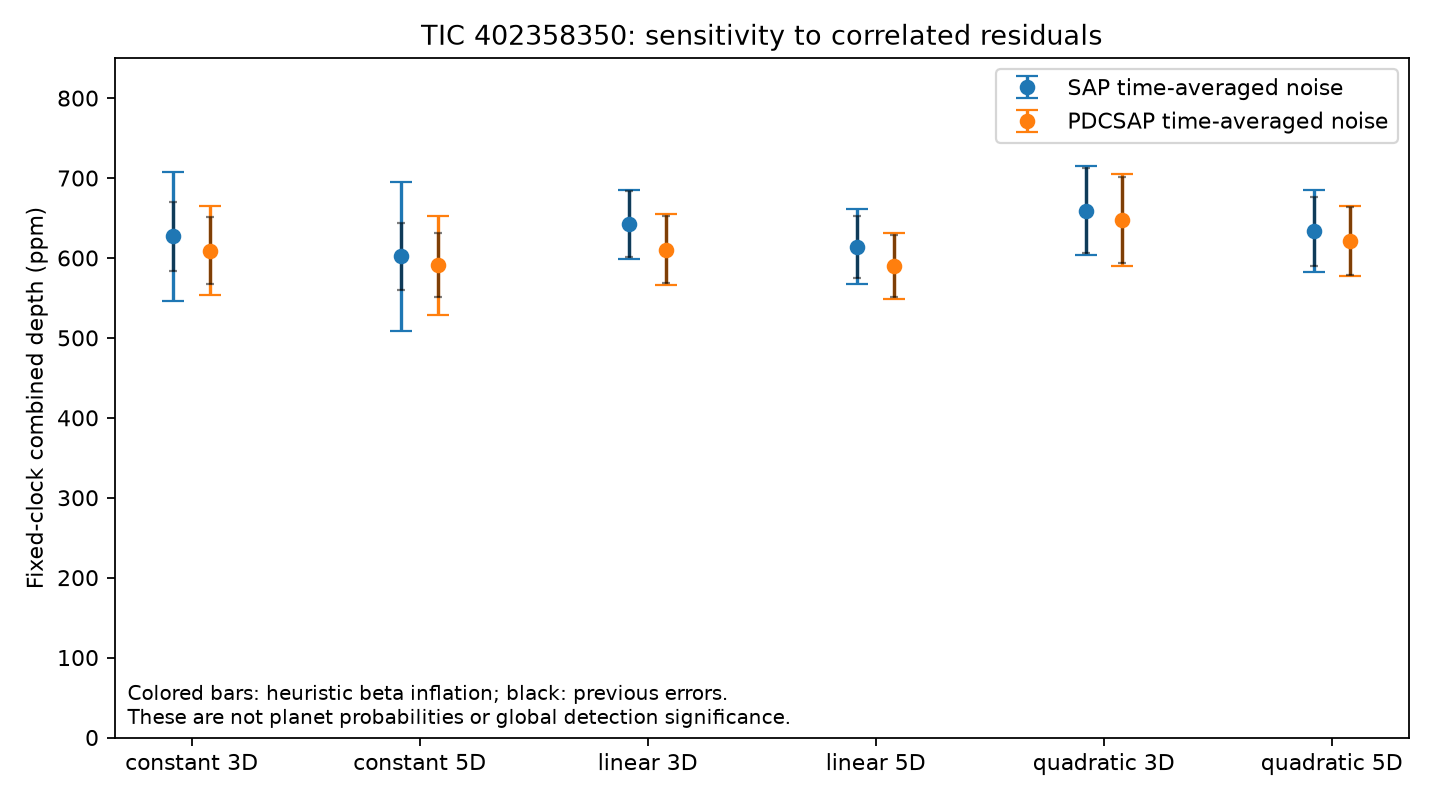
\includegraphics[width=\linewidth,height=0.72\textheight,keepaspectratio]{figures/402-noise.png}
\caption{TIC 402358350 noise sensitivity across the twelve SAP/PDC baseline methods. Missing or insufficiently populated time bins remain unavailable; the combined error range is 41--93 ppm. Reweighting the events is a separately labeled sensitivity test. These methods reuse the same eight events.}
\end{figure}
\begin{figure}[p]
\centering
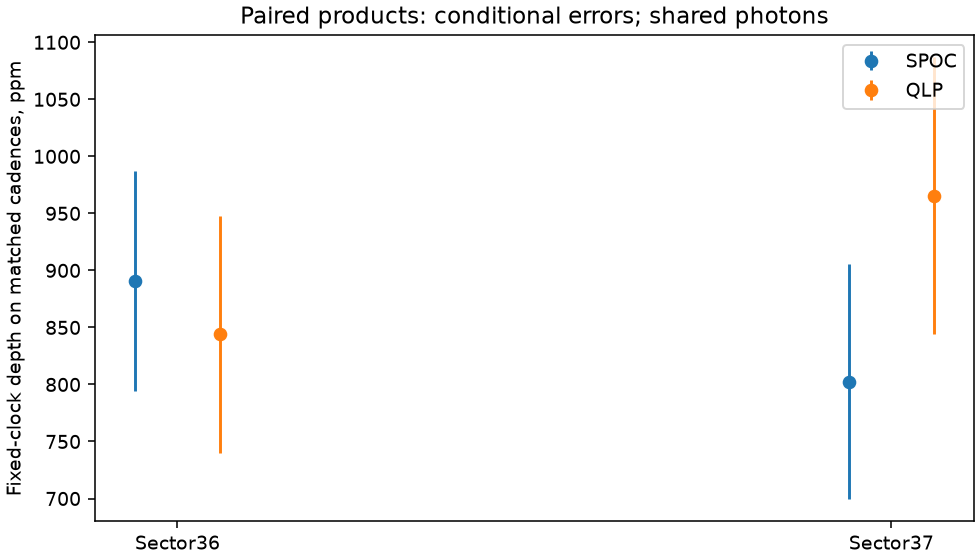
\includegraphics[width=\linewidth,height=0.72\textheight,keepaspectratio]{figures/803-paired.png}
\caption{TIC 80387959 paired SPOC/QLP reductions of the same sector-36/37 exposures. Differences depend on epoch and common-quality selection. They do not establish a universal QLP depth suppression or physical depth evolution.}
\end{figure}
\begin{figure}[p]
\centering
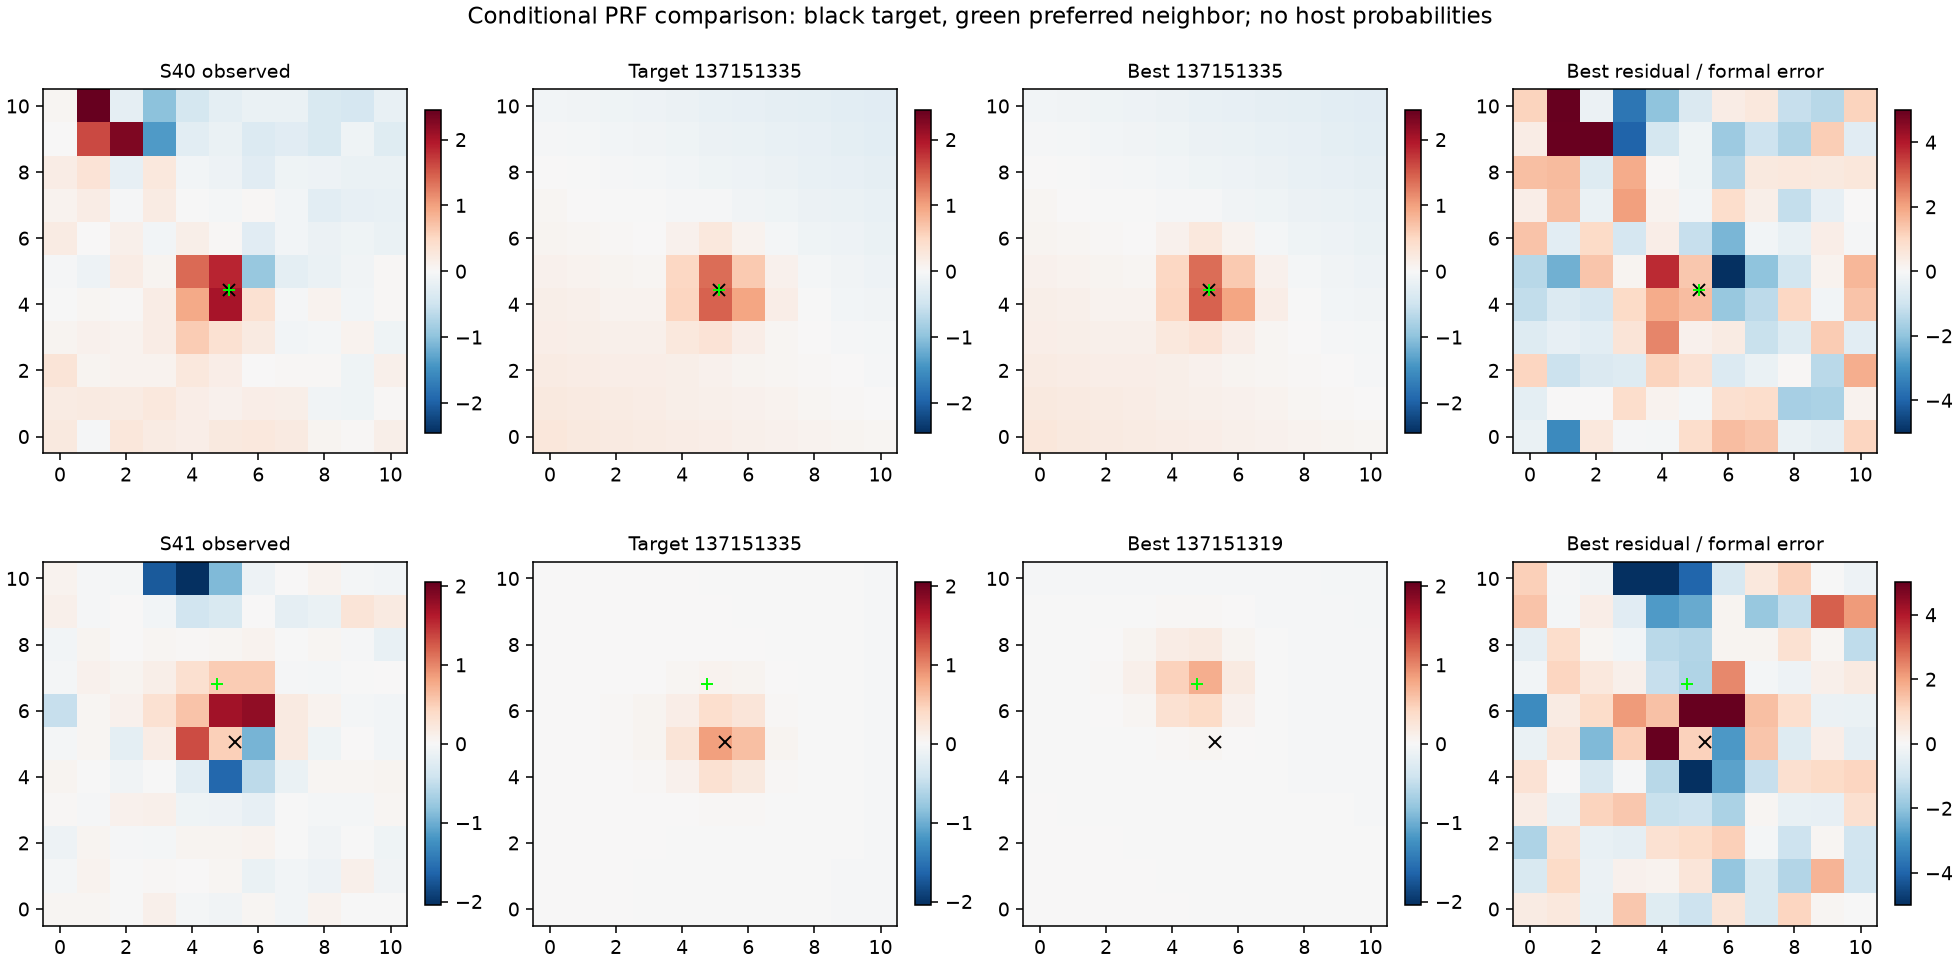
\includegraphics[width=\linewidth,height=0.72\textheight,keepaspectratio]{figures/host-control.png}
\caption{Known-host Kepler-93 b image control. The original template method prefers the correct target in sector 40 and a neighbor in sector 41 despite the established planetary signal. Structured residuals and wrong rankings undermine a probability interpretation of the same method on the candidates.}
\end{figure}
\begin{figure}[p]
\centering
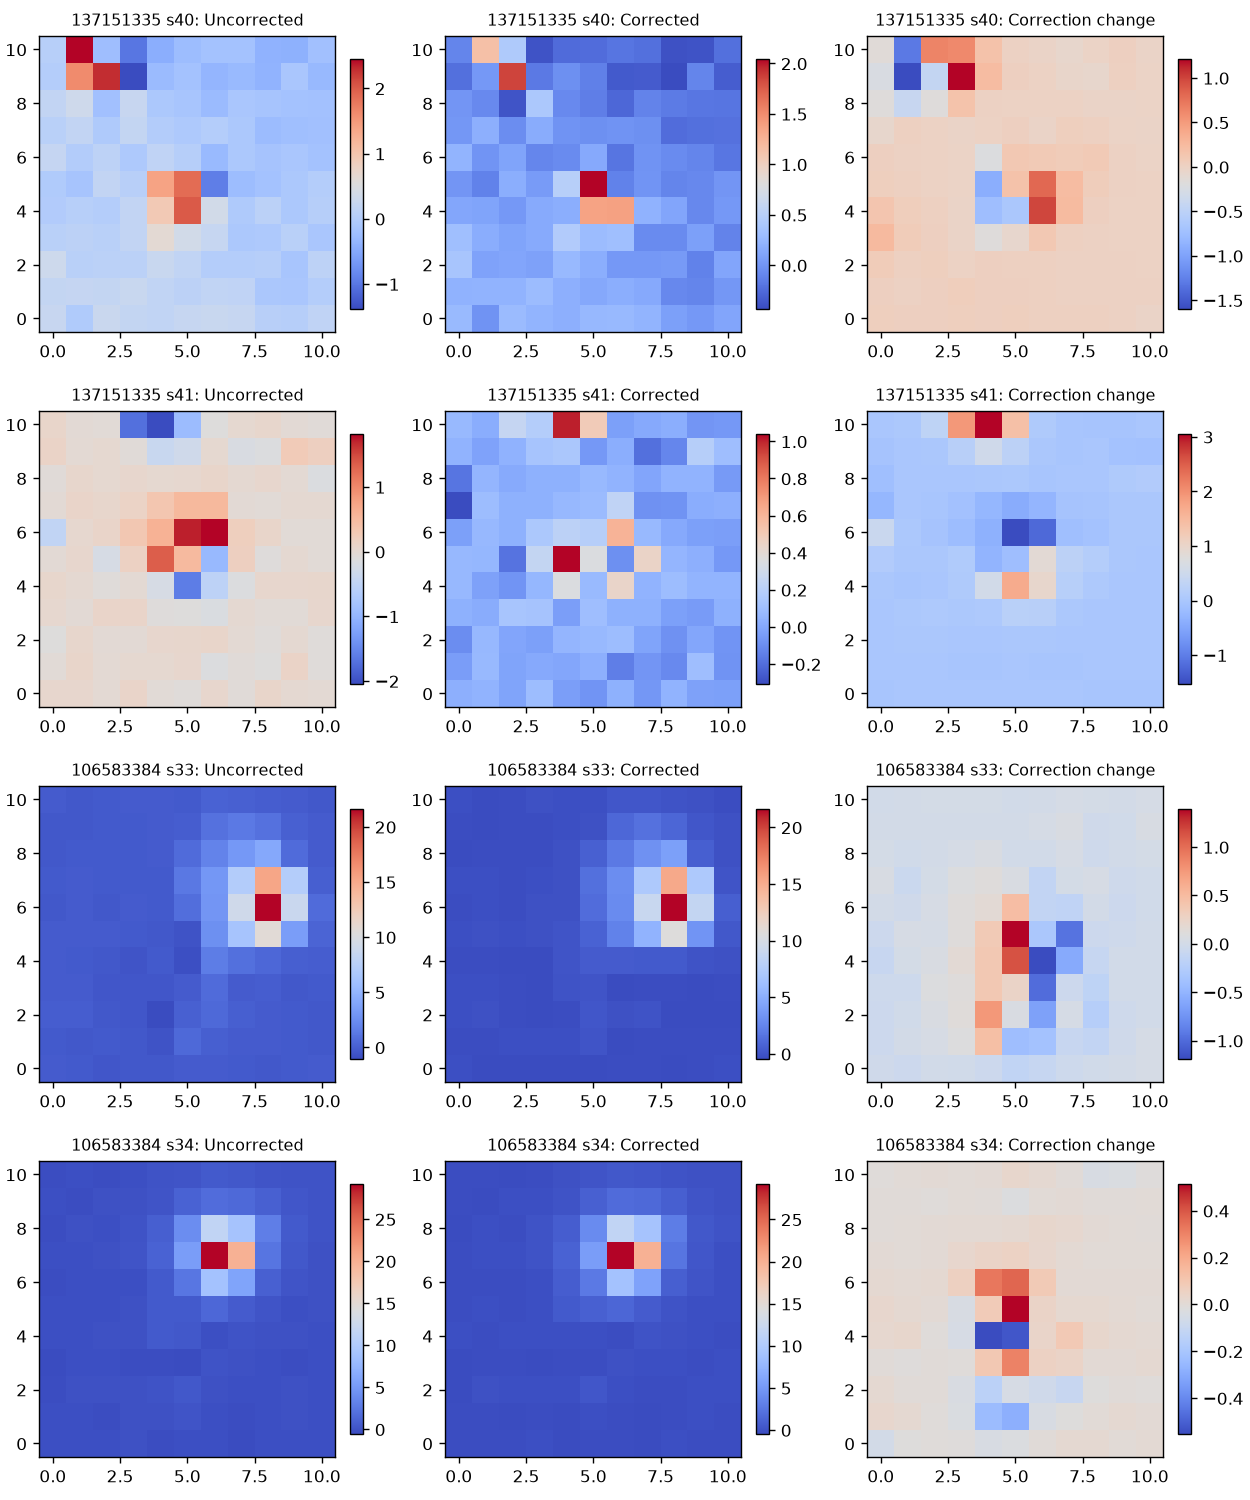
\includegraphics[width=\linewidth,height=0.72\textheight,keepaspectratio]{figures/controls-pointing.png}
\caption{Pointing-correction controls: three of four satisfy the frozen criterion. The Kepler-93 wrong-host case improves, but discrimination decreases in one contaminant sector. The complete gate therefore fails and the method is not applied to infer candidate hosts.}
\end{figure}
\begin{figure}[p]
\centering
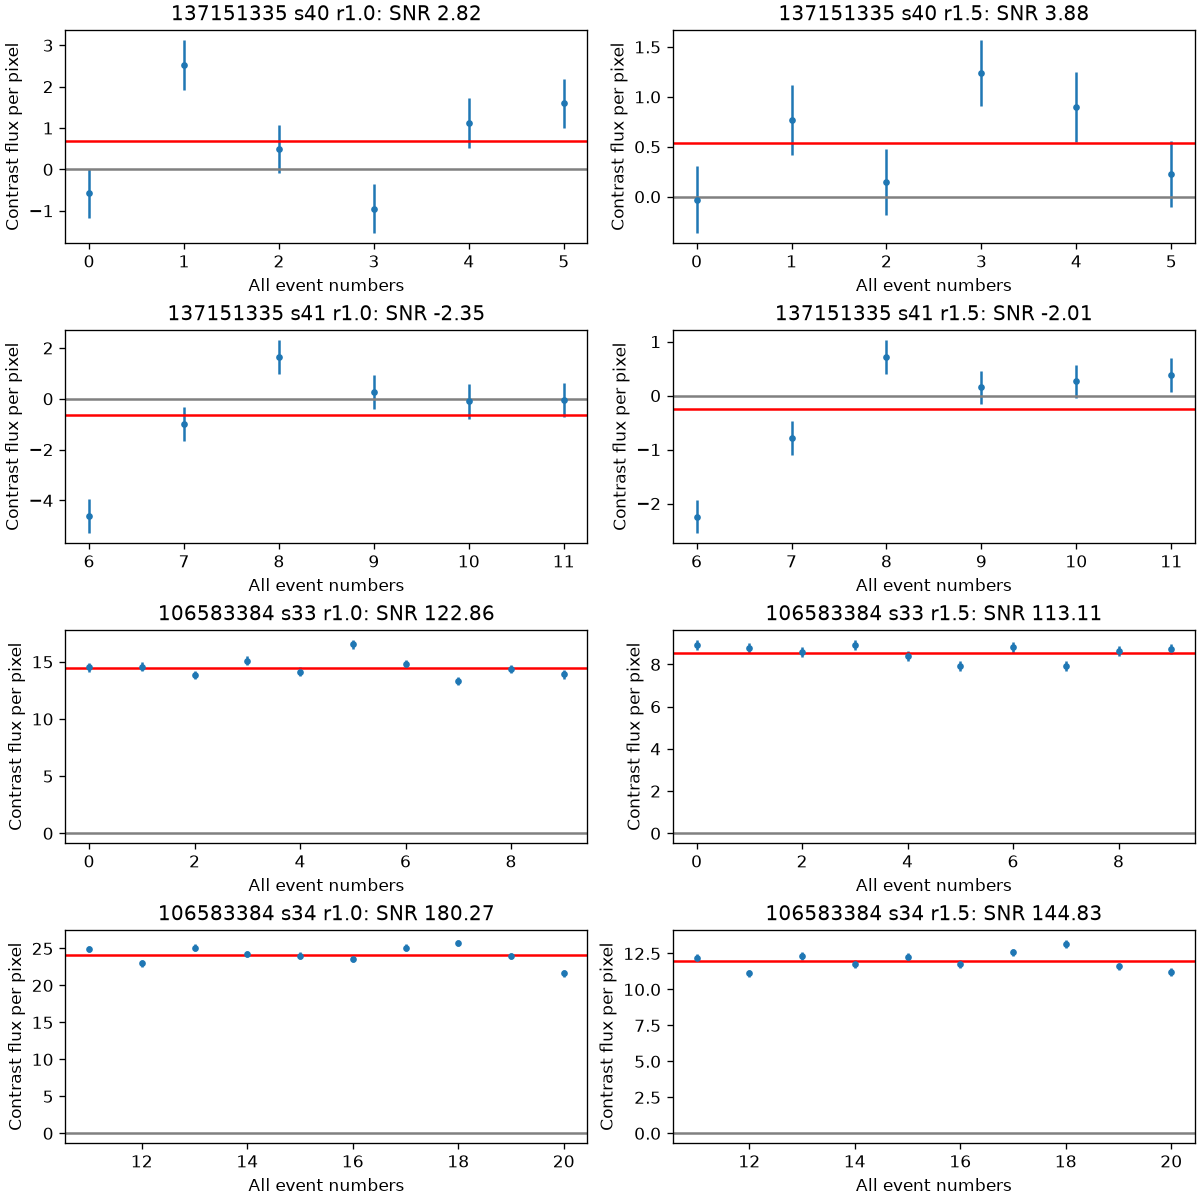
\includegraphics[width=\linewidth,height=0.72\textheight,keepaspectratio]{figures/controls-aperture.png}
\caption{Paired-aperture controls: five of eight sector/radius cases pass. Kepler-93 failures include a weak target measurement and wrong-region contrasts. The ordinate measures differential variable flux per exclusive pixel, not stellar fractional eclipse depth or calibrated throughput. The candidate-application gate fails.}
\end{figure}
\begin{figure}[p]
\centering
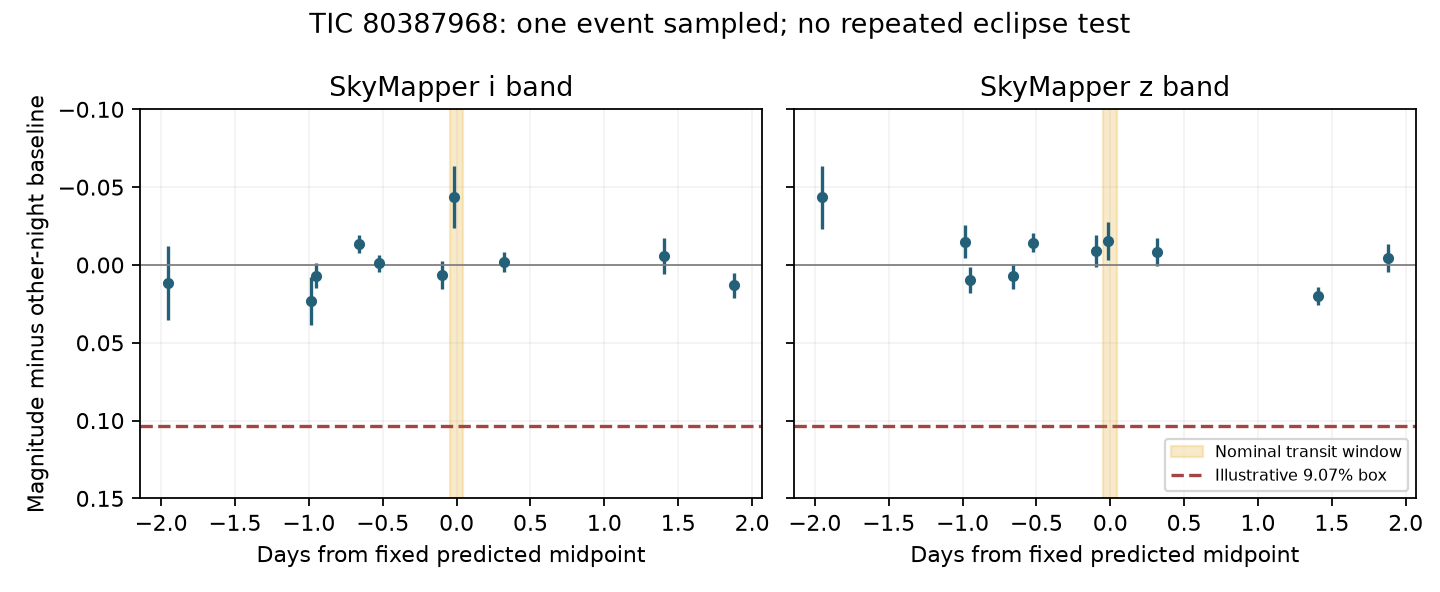
\includegraphics[width=\linewidth,height=0.72\textheight,keepaspectratio]{figures/803-resolved.png}
\caption{Resolved SkyMapper samples for neighbor TIC 80387968. Two measurements in different filters sample one predicted event without dimming, weakening a specified same-depth eclipse at those instants. The required two-event exclusion gate fails; sparse color-dependent samples do not clear the neighbor.}
\end{figure}
\begin{figure}[p]
\centering
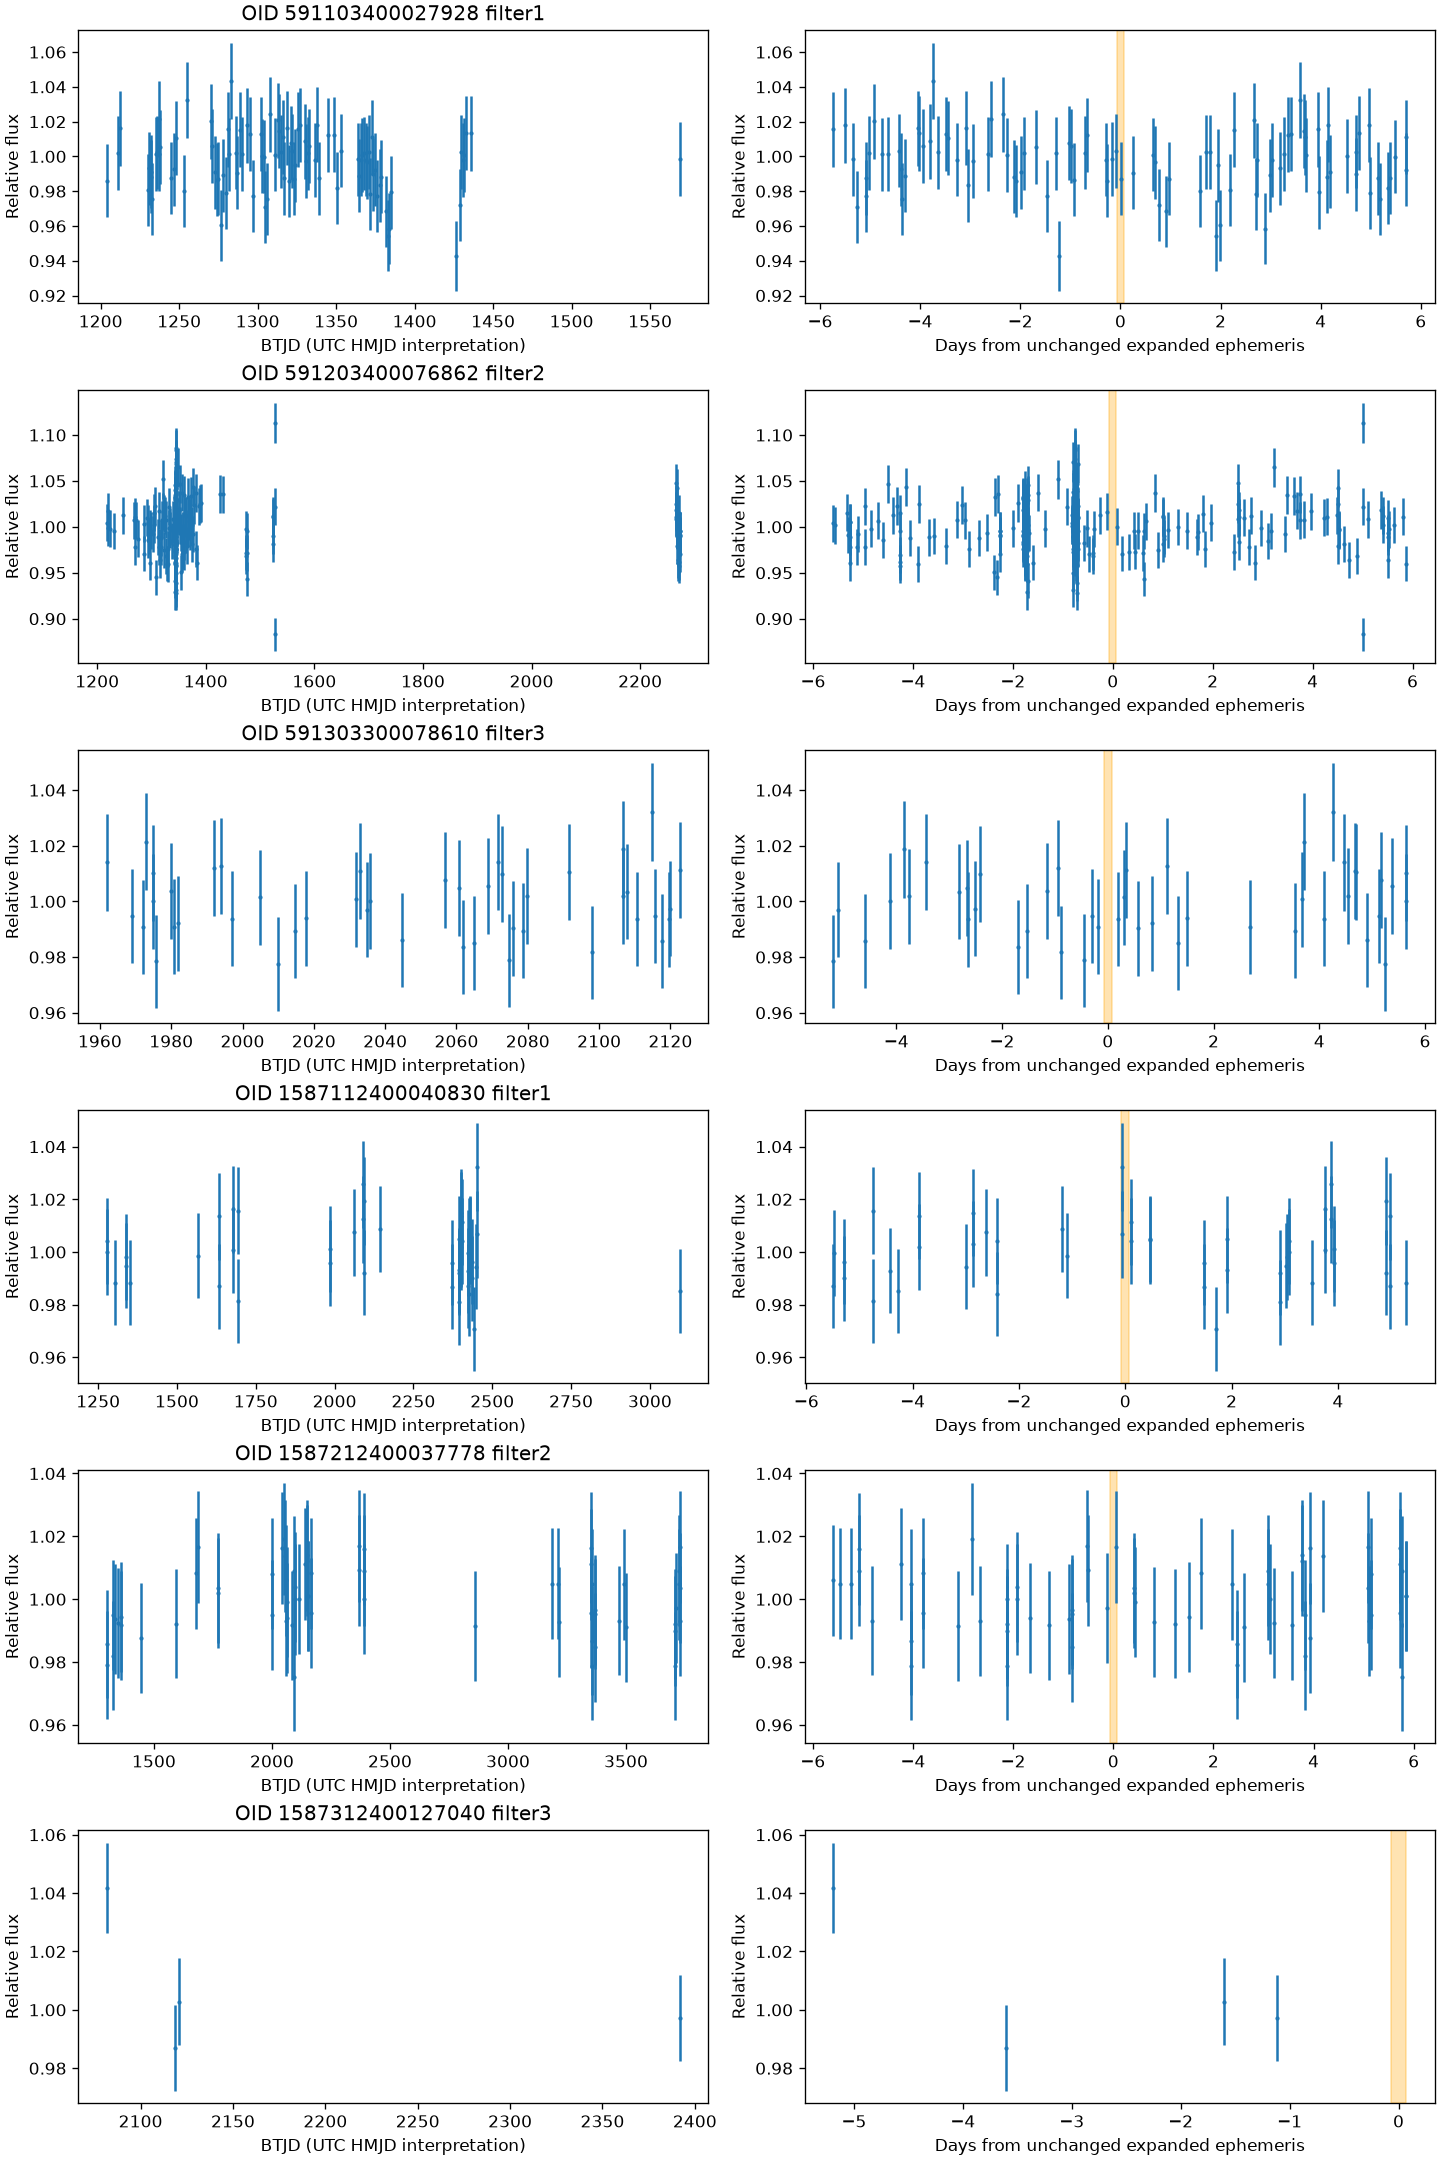
\includegraphics[width=\linewidth,height=0.72\textheight,keepaspectratio]{figures/402-resolved.png}
\caption{Resolved ZTF measurements for neighbor TIC 74037550 near TIC 402358350. Six streams contain 836 retrieved and 545 quality-selected points. All 72 clock/time-convention/stream-or-filter comparisons remain inconclusive; these plots provide neither a recovered eclipse nor a neighbor exclusion.}
\end{figure}
\begin{figure}[p]
\centering
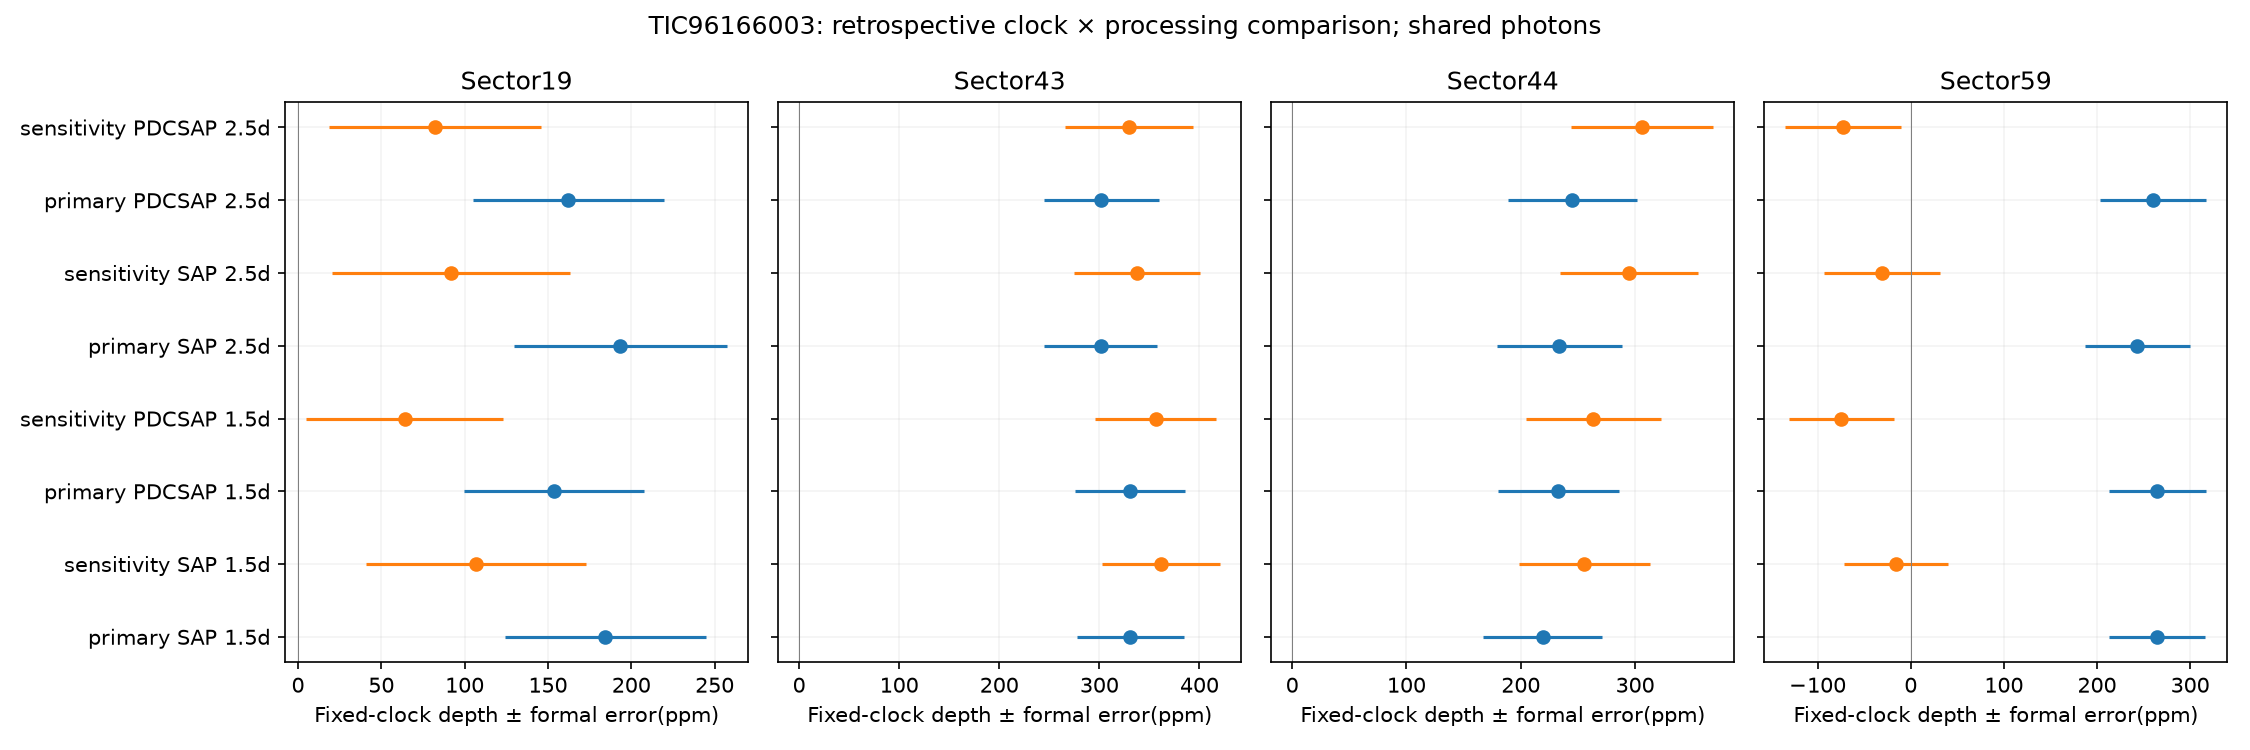
\includegraphics[width=\linewidth,height=0.72\textheight,keepaspectratio]{figures/961-clocks.png}
\caption{Crossed clock and processing comparison for TIC 96166003 sector 59. The expanded primary clock retains dimming across SAP/PDC and two detrending choices, whereas its alternative is negative or near zero. Shared-photon processing agreement does not identify the correct clock, and the original prediction timing remains inadequate.}
\end{figure}
\begin{figure}[p]
\centering
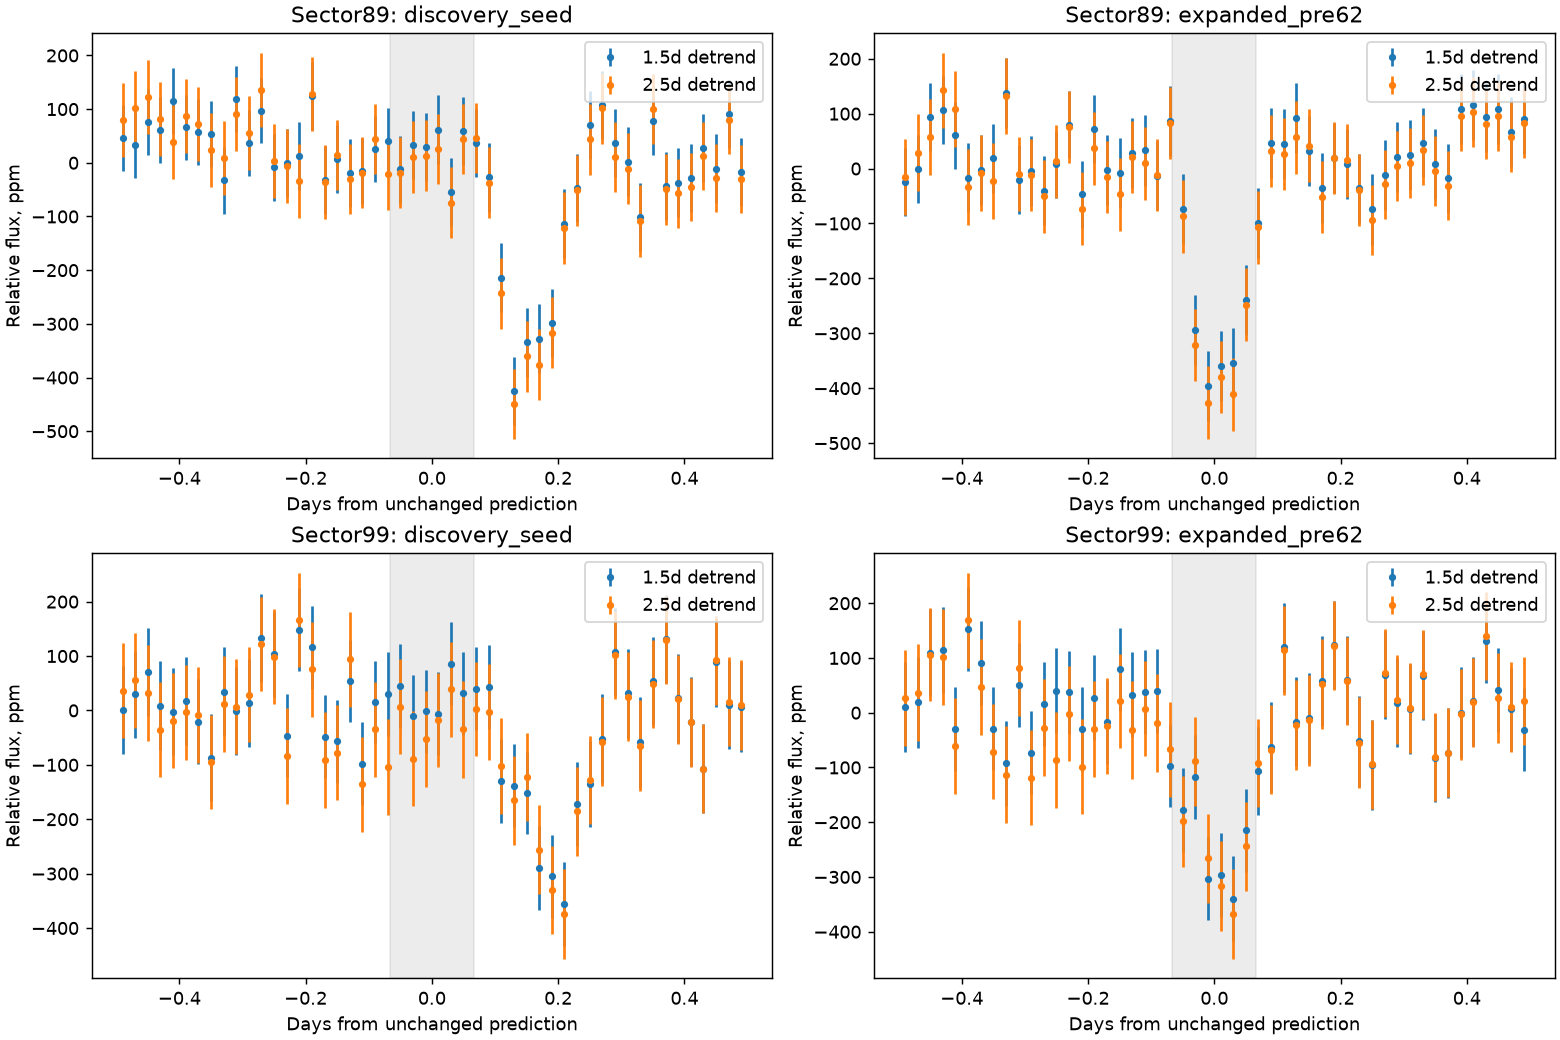
\includegraphics[width=\linewidth,height=0.72\textheight,keepaspectratio]{figures/554-new.png}
\caption{TIC 5546257 sectors 89 and 99 at the saved clock alternatives. Expanded-clock dips remain positive but fail the original timing gate; the coarse seed is unfavorable. Extraction and aperture differences limit physical depth comparisons. Neighbor Gaia variability strengthens contamination independently of these blended reductions.}
\end{figure}
\clearpage

\end{document}
